\documentclass{article}

    % This code is generated
    \usepackage[breakable]{tcolorbox}
    \usepackage{parskip} % Stop auto-indenting (to mimic markdown behaviour)
    

    % Basic figure setup, for now with no caption control since it's done
    % automatically by Pandoc (which extracts ![](path) syntax from Markdown).
    \usepackage{graphicx}
    % Maintain compatibility with old templates. Remove in nbconvert 6.0
    \let\Oldincludegraphics\includegraphics
    % Ensure that by default, figures have no caption (until we provide a
    % proper Figure object with a Caption API and a way to capture that
    % in the conversion process - todo).
    \usepackage{caption}
    \DeclareCaptionFormat{nocaption}{}
    \captionsetup{format=nocaption,aboveskip=0pt,belowskip=0pt}

    \usepackage{float}
    \floatplacement{figure}{H} % forces figures to be placed at the correct location
    \usepackage{xcolor} % Allow colors to be defined
    \usepackage{enumerate} % Needed for markdown enumerations to work
    \usepackage[left=2cm,right=2cm, top=2cm,bottom=2cm,bindingoffset=0cm]{geometry}
    % \usepackage{geometry} % Used to adjust the document margins
    \usepackage{amsmath} % Equations
    \usepackage{amssymb} % Equations
    \usepackage{textcomp} % defines textquotesingle
    % Hack from http://tex.stackexchange.com/a/47451/13684:
    \AtBeginDocument{%
        \def\PYZsq{\textquotesingle}% Upright quotes in Pygmentized code
    }
    \usepackage{upquote} % Upright quotes for verbatim code
    \usepackage{eurosym} % defines \euro

    \usepackage{iftex}
    \ifPDFTeX
        \usepackage[T1]{fontenc}
        \IfFileExists{alphabeta.sty}{
              \usepackage{alphabeta}
          }{
              \usepackage[mathletters]{ucs}
              % \usepackage[utf8x]{inputenc}
          }
    \else
        \usepackage{fontspec}
        \usepackage{unicode-math}
    \fi

    \usepackage{fancyvrb} % verbatim replacement that allows latex
    \usepackage{grffile} % extends the file name processing of package graphics
                         % to support a larger range
    \makeatletter % fix for old versions of grffile with XeLaTeX
    \@ifpackagelater{grffile}{2019/11/01}
    {
      % Do nothing on new versions
    }
    {
      \def\Gread@@xetex#1{%
        \IfFileExists{"\Gin@base".bb}%
        {\Gread@eps{\Gin@base.bb}}%
        {\Gread@@xetex@aux#1}%
      }
    }
    \makeatother
    \usepackage[Export]{adjustbox} % Used to constrain images to a maximum size
    \adjustboxset{max size={0.9\linewidth}{0.9\paperheight}}

    % The hyperref package gives us a pdf with properly built
    % internal navigation ('pdf bookmarks' for the table of contents,
    % internal cross-reference links, web links for URLs, etc.)
    \usepackage{hyperref}
    % The default LaTeX title has an obnoxious amount of whitespace. By default,
    % titling removes some of it. It also provides customization options.
    \usepackage{titling}
    \usepackage{longtable} % longtable support required by pandoc >1.10
    \usepackage{booktabs}  % table support for pandoc > 1.12.2
    \usepackage{array}     % table support for pandoc >= 2.11.3
    \usepackage{calc}      % table minipage width calculation for pandoc >= 2.11.1
    \usepackage[inline]{enumitem} % IRkernel/repr support (it uses the enumerate* environment)
    \usepackage[normalem]{ulem} % ulem is needed to support strikethroughs (\sout)
                                % normalem makes italics be italics, not underlines
    \usepackage{soul}      % strikethrough (\st) support for pandoc >= 3.0.0
    \usepackage{mathrsfs}
    

    
    % Colors for the hyperref package
    \definecolor{urlcolor}{rgb}{0,.145,.698}
    \definecolor{linkcolor}{rgb}{.71,0.21,0.01}
    \definecolor{citecolor}{rgb}{.12,.54,.11}

    % ANSI colors
    \definecolor{ansi-black}{HTML}{3E424D}
    \definecolor{ansi-black-intense}{HTML}{282C36}
    \definecolor{ansi-red}{HTML}{E75C58}
    \definecolor{ansi-red-intense}{HTML}{B22B31}
    \definecolor{ansi-green}{HTML}{00A250}
    \definecolor{ansi-green-intense}{HTML}{007427}
    \definecolor{ansi-yellow}{HTML}{DDB62B}
    \definecolor{ansi-yellow-intense}{HTML}{B27D12}
    \definecolor{ansi-blue}{HTML}{208FFB}
    \definecolor{ansi-blue-intense}{HTML}{0065CA}
    \definecolor{ansi-magenta}{HTML}{D160C4}
    \definecolor{ansi-magenta-intense}{HTML}{A03196}
    \definecolor{ansi-cyan}{HTML}{60C6C8}
    \definecolor{ansi-cyan-intense}{HTML}{258F8F}
    \definecolor{ansi-white}{HTML}{C5C1B4}
    \definecolor{ansi-white-intense}{HTML}{A1A6B2}
    \definecolor{ansi-default-inverse-fg}{HTML}{FFFFFF}
    \definecolor{ansi-default-inverse-bg}{HTML}{000000}

    % common color for the border for error outputs.
    \definecolor{outerrorbackground}{HTML}{FFDFDF}

    % commands and environments needed by pandoc snippets
    % extracted from the output of `pandoc -s`
    \providecommand{\tightlist}{%
      \setlength{\itemsep}{0pt}\setlength{\parskip}{0pt}}
    \DefineVerbatimEnvironment{Highlighting}{Verbatim}{commandchars=\\\{\}}
    % Add ',fontsize=\small' for more characters per line
    \newenvironment{Shaded}{}{}
    \newcommand{\KeywordTok}[1]{\textcolor[rgb]{0.00,0.44,0.13}{\textbf{{#1}}}}
    \newcommand{\DataTypeTok}[1]{\textcolor[rgb]{0.56,0.13,0.00}{{#1}}}
    \newcommand{\DecValTok}[1]{\textcolor[rgb]{0.25,0.63,0.44}{{#1}}}
    \newcommand{\BaseNTok}[1]{\textcolor[rgb]{0.25,0.63,0.44}{{#1}}}
    \newcommand{\FloatTok}[1]{\textcolor[rgb]{0.25,0.63,0.44}{{#1}}}
    \newcommand{\CharTok}[1]{\textcolor[rgb]{0.25,0.44,0.63}{{#1}}}
    \newcommand{\StringTok}[1]{\textcolor[rgb]{0.25,0.44,0.63}{{#1}}}
    \newcommand{\CommentTok}[1]{\textcolor[rgb]{0.38,0.63,0.69}{\textit{{#1}}}}
    \newcommand{\OtherTok}[1]{\textcolor[rgb]{0.00,0.44,0.13}{{#1}}}
    \newcommand{\AlertTok}[1]{\textcolor[rgb]{1.00,0.00,0.00}{\textbf{{#1}}}}
    \newcommand{\FunctionTok}[1]{\textcolor[rgb]{0.02,0.16,0.49}{{#1}}}
    \newcommand{\RegionMarkerTok}[1]{{#1}}
    \newcommand{\ErrorTok}[1]{\textcolor[rgb]{1.00,0.00,0.00}{\textbf{{#1}}}}
    \newcommand{\NormalTok}[1]{{#1}}

    % Additional commands for more recent versions of Pandoc
    \newcommand{\ConstantTok}[1]{\textcolor[rgb]{0.53,0.00,0.00}{{#1}}}
    \newcommand{\SpecialCharTok}[1]{\textcolor[rgb]{0.25,0.44,0.63}{{#1}}}
    \newcommand{\VerbatimStringTok}[1]{\textcolor[rgb]{0.25,0.44,0.63}{{#1}}}
    \newcommand{\SpecialStringTok}[1]{\textcolor[rgb]{0.73,0.40,0.53}{{#1}}}
    \newcommand{\ImportTok}[1]{{#1}}
    \newcommand{\DocumentationTok}[1]{\textcolor[rgb]{0.73,0.13,0.13}{\textit{{#1}}}}
    \newcommand{\AnnotationTok}[1]{\textcolor[rgb]{0.38,0.63,0.69}{\textbf{\textit{{#1}}}}}
    \newcommand{\CommentVarTok}[1]{\textcolor[rgb]{0.38,0.63,0.69}{\textbf{\textit{{#1}}}}}
    \newcommand{\VariableTok}[1]{\textcolor[rgb]{0.10,0.09,0.49}{{#1}}}
    \newcommand{\ControlFlowTok}[1]{\textcolor[rgb]{0.00,0.44,0.13}{\textbf{{#1}}}}
    \newcommand{\OperatorTok}[1]{\textcolor[rgb]{0.40,0.40,0.40}{{#1}}}
    \newcommand{\BuiltInTok}[1]{{#1}}
    \newcommand{\ExtensionTok}[1]{{#1}}
    \newcommand{\PreprocessorTok}[1]{\textcolor[rgb]{0.74,0.48,0.00}{{#1}}}
    \newcommand{\AttributeTok}[1]{\textcolor[rgb]{0.49,0.56,0.16}{{#1}}}
    \newcommand{\InformationTok}[1]{\textcolor[rgb]{0.38,0.63,0.69}{\textbf{\textit{{#1}}}}}
    \newcommand{\WarningTok}[1]{\textcolor[rgb]{0.38,0.63,0.69}{\textbf{\textit{{#1}}}}}


    % Define a nice break command that doesn't care if a line doesn't already
    % exist.
    \def\br{\hspace*{\fill} \\* }
    % Math Jax compatibility definitions
    \def\gt{>}
    \def\lt{<}
    \let\Oldtex\TeX
    \let\Oldlatex\LaTeX
    \renewcommand{\TeX}{\textrm{\Oldtex}}
    \renewcommand{\LaTeX}{\textrm{\Oldlatex}}
    % Document parameters
    % Document title
    \title{Automatic Differentiation}
    
    
    
    
    
    
    
% Pygments definitions
\makeatletter
\def\PY@reset{\let\PY@it=\relax \let\PY@bf=\relax%
    \let\PY@ul=\relax \let\PY@tc=\relax%
    \let\PY@bc=\relax \let\PY@ff=\relax}
\def\PY@tok#1{\csname PY@tok@#1\endcsname}
\def\PY@toks#1+{\ifx\relax#1\empty\else%
    \PY@tok{#1}\expandafter\PY@toks\fi}
\def\PY@do#1{\PY@bc{\PY@tc{\PY@ul{%
    \PY@it{\PY@bf{\PY@ff{#1}}}}}}}
\def\PY#1#2{\PY@reset\PY@toks#1+\relax+\PY@do{#2}}

\@namedef{PY@tok@w}{\def\PY@tc##1{\textcolor[rgb]{0.73,0.73,0.73}{##1}}}
\@namedef{PY@tok@c}{\let\PY@it=\textit\def\PY@tc##1{\textcolor[rgb]{0.24,0.48,0.48}{##1}}}
\@namedef{PY@tok@cp}{\def\PY@tc##1{\textcolor[rgb]{0.61,0.40,0.00}{##1}}}
\@namedef{PY@tok@k}{\let\PY@bf=\textbf\def\PY@tc##1{\textcolor[rgb]{0.00,0.50,0.00}{##1}}}
\@namedef{PY@tok@kp}{\def\PY@tc##1{\textcolor[rgb]{0.00,0.50,0.00}{##1}}}
\@namedef{PY@tok@kt}{\def\PY@tc##1{\textcolor[rgb]{0.69,0.00,0.25}{##1}}}
\@namedef{PY@tok@o}{\def\PY@tc##1{\textcolor[rgb]{0.40,0.40,0.40}{##1}}}
\@namedef{PY@tok@ow}{\let\PY@bf=\textbf\def\PY@tc##1{\textcolor[rgb]{0.67,0.13,1.00}{##1}}}
\@namedef{PY@tok@nb}{\def\PY@tc##1{\textcolor[rgb]{0.00,0.50,0.00}{##1}}}
\@namedef{PY@tok@nf}{\def\PY@tc##1{\textcolor[rgb]{0.00,0.00,1.00}{##1}}}
\@namedef{PY@tok@nc}{\let\PY@bf=\textbf\def\PY@tc##1{\textcolor[rgb]{0.00,0.00,1.00}{##1}}}
\@namedef{PY@tok@nn}{\let\PY@bf=\textbf\def\PY@tc##1{\textcolor[rgb]{0.00,0.00,1.00}{##1}}}
\@namedef{PY@tok@ne}{\let\PY@bf=\textbf\def\PY@tc##1{\textcolor[rgb]{0.80,0.25,0.22}{##1}}}
\@namedef{PY@tok@nv}{\def\PY@tc##1{\textcolor[rgb]{0.10,0.09,0.49}{##1}}}
\@namedef{PY@tok@no}{\def\PY@tc##1{\textcolor[rgb]{0.53,0.00,0.00}{##1}}}
\@namedef{PY@tok@nl}{\def\PY@tc##1{\textcolor[rgb]{0.46,0.46,0.00}{##1}}}
\@namedef{PY@tok@ni}{\let\PY@bf=\textbf\def\PY@tc##1{\textcolor[rgb]{0.44,0.44,0.44}{##1}}}
\@namedef{PY@tok@na}{\def\PY@tc##1{\textcolor[rgb]{0.41,0.47,0.13}{##1}}}
\@namedef{PY@tok@nt}{\let\PY@bf=\textbf\def\PY@tc##1{\textcolor[rgb]{0.00,0.50,0.00}{##1}}}
\@namedef{PY@tok@nd}{\def\PY@tc##1{\textcolor[rgb]{0.67,0.13,1.00}{##1}}}
\@namedef{PY@tok@s}{\def\PY@tc##1{\textcolor[rgb]{0.73,0.13,0.13}{##1}}}
\@namedef{PY@tok@sd}{\let\PY@it=\textit\def\PY@tc##1{\textcolor[rgb]{0.73,0.13,0.13}{##1}}}
\@namedef{PY@tok@si}{\let\PY@bf=\textbf\def\PY@tc##1{\textcolor[rgb]{0.64,0.35,0.47}{##1}}}
\@namedef{PY@tok@se}{\let\PY@bf=\textbf\def\PY@tc##1{\textcolor[rgb]{0.67,0.36,0.12}{##1}}}
\@namedef{PY@tok@sr}{\def\PY@tc##1{\textcolor[rgb]{0.64,0.35,0.47}{##1}}}
\@namedef{PY@tok@ss}{\def\PY@tc##1{\textcolor[rgb]{0.10,0.09,0.49}{##1}}}
\@namedef{PY@tok@sx}{\def\PY@tc##1{\textcolor[rgb]{0.00,0.50,0.00}{##1}}}
\@namedef{PY@tok@m}{\def\PY@tc##1{\textcolor[rgb]{0.40,0.40,0.40}{##1}}}
\@namedef{PY@tok@gh}{\let\PY@bf=\textbf\def\PY@tc##1{\textcolor[rgb]{0.00,0.00,0.50}{##1}}}
\@namedef{PY@tok@gu}{\let\PY@bf=\textbf\def\PY@tc##1{\textcolor[rgb]{0.50,0.00,0.50}{##1}}}
\@namedef{PY@tok@gd}{\def\PY@tc##1{\textcolor[rgb]{0.63,0.00,0.00}{##1}}}
\@namedef{PY@tok@gi}{\def\PY@tc##1{\textcolor[rgb]{0.00,0.52,0.00}{##1}}}
\@namedef{PY@tok@gr}{\def\PY@tc##1{\textcolor[rgb]{0.89,0.00,0.00}{##1}}}
\@namedef{PY@tok@ge}{\let\PY@it=\textit}
\@namedef{PY@tok@gs}{\let\PY@bf=\textbf}
\@namedef{PY@tok@ges}{\let\PY@bf=\textbf\let\PY@it=\textit}
\@namedef{PY@tok@gp}{\let\PY@bf=\textbf\def\PY@tc##1{\textcolor[rgb]{0.00,0.00,0.50}{##1}}}
\@namedef{PY@tok@go}{\def\PY@tc##1{\textcolor[rgb]{0.44,0.44,0.44}{##1}}}
\@namedef{PY@tok@gt}{\def\PY@tc##1{\textcolor[rgb]{0.00,0.27,0.87}{##1}}}
\@namedef{PY@tok@err}{\def\PY@bc##1{{\setlength{\fboxsep}{\string -\fboxrule}\fcolorbox[rgb]{1.00,0.00,0.00}{1,1,1}{\strut ##1}}}}
\@namedef{PY@tok@kc}{\let\PY@bf=\textbf\def\PY@tc##1{\textcolor[rgb]{0.00,0.50,0.00}{##1}}}
\@namedef{PY@tok@kd}{\let\PY@bf=\textbf\def\PY@tc##1{\textcolor[rgb]{0.00,0.50,0.00}{##1}}}
\@namedef{PY@tok@kn}{\let\PY@bf=\textbf\def\PY@tc##1{\textcolor[rgb]{0.00,0.50,0.00}{##1}}}
\@namedef{PY@tok@kr}{\let\PY@bf=\textbf\def\PY@tc##1{\textcolor[rgb]{0.00,0.50,0.00}{##1}}}
\@namedef{PY@tok@bp}{\def\PY@tc##1{\textcolor[rgb]{0.00,0.50,0.00}{##1}}}
\@namedef{PY@tok@fm}{\def\PY@tc##1{\textcolor[rgb]{0.00,0.00,1.00}{##1}}}
\@namedef{PY@tok@vc}{\def\PY@tc##1{\textcolor[rgb]{0.10,0.09,0.49}{##1}}}
\@namedef{PY@tok@vg}{\def\PY@tc##1{\textcolor[rgb]{0.10,0.09,0.49}{##1}}}
\@namedef{PY@tok@vi}{\def\PY@tc##1{\textcolor[rgb]{0.10,0.09,0.49}{##1}}}
\@namedef{PY@tok@vm}{\def\PY@tc##1{\textcolor[rgb]{0.10,0.09,0.49}{##1}}}
\@namedef{PY@tok@sa}{\def\PY@tc##1{\textcolor[rgb]{0.73,0.13,0.13}{##1}}}
\@namedef{PY@tok@sb}{\def\PY@tc##1{\textcolor[rgb]{0.73,0.13,0.13}{##1}}}
\@namedef{PY@tok@sc}{\def\PY@tc##1{\textcolor[rgb]{0.73,0.13,0.13}{##1}}}
\@namedef{PY@tok@dl}{\def\PY@tc##1{\textcolor[rgb]{0.73,0.13,0.13}{##1}}}
\@namedef{PY@tok@s2}{\def\PY@tc##1{\textcolor[rgb]{0.73,0.13,0.13}{##1}}}
\@namedef{PY@tok@sh}{\def\PY@tc##1{\textcolor[rgb]{0.73,0.13,0.13}{##1}}}
\@namedef{PY@tok@s1}{\def\PY@tc##1{\textcolor[rgb]{0.73,0.13,0.13}{##1}}}
\@namedef{PY@tok@mb}{\def\PY@tc##1{\textcolor[rgb]{0.40,0.40,0.40}{##1}}}
\@namedef{PY@tok@mf}{\def\PY@tc##1{\textcolor[rgb]{0.40,0.40,0.40}{##1}}}
\@namedef{PY@tok@mh}{\def\PY@tc##1{\textcolor[rgb]{0.40,0.40,0.40}{##1}}}
\@namedef{PY@tok@mi}{\def\PY@tc##1{\textcolor[rgb]{0.40,0.40,0.40}{##1}}}
\@namedef{PY@tok@il}{\def\PY@tc##1{\textcolor[rgb]{0.40,0.40,0.40}{##1}}}
\@namedef{PY@tok@mo}{\def\PY@tc##1{\textcolor[rgb]{0.40,0.40,0.40}{##1}}}
\@namedef{PY@tok@ch}{\let\PY@it=\textit\def\PY@tc##1{\textcolor[rgb]{0.24,0.48,0.48}{##1}}}
\@namedef{PY@tok@cm}{\let\PY@it=\textit\def\PY@tc##1{\textcolor[rgb]{0.24,0.48,0.48}{##1}}}
\@namedef{PY@tok@cpf}{\let\PY@it=\textit\def\PY@tc##1{\textcolor[rgb]{0.24,0.48,0.48}{##1}}}
\@namedef{PY@tok@c1}{\let\PY@it=\textit\def\PY@tc##1{\textcolor[rgb]{0.24,0.48,0.48}{##1}}}
\@namedef{PY@tok@cs}{\let\PY@it=\textit\def\PY@tc##1{\textcolor[rgb]{0.24,0.48,0.48}{##1}}}

\def\PYZbs{\char`\\}
\def\PYZus{\char`\_}
\def\PYZob{\char`\{}
\def\PYZcb{\char`\}}
\def\PYZca{\char`\^}
\def\PYZam{\char`\&}
\def\PYZlt{\char`\<}
\def\PYZgt{\char`\>}
\def\PYZsh{\char`\#}
\def\PYZpc{\char`\%}
\def\PYZdl{\char`\$}
\def\PYZhy{\char`\-}
\def\PYZsq{\char`\'}
\def\PYZdq{\char`\"}
\def\PYZti{\char`\~}
% for compatibility with earlier versions
\def\PYZat{@}
\def\PYZlb{[}
\def\PYZrb{]}
\makeatother


    % For linebreaks inside Verbatim environment from package fancyvrb.
    \makeatletter
        \newbox\Wrappedcontinuationbox
        \newbox\Wrappedvisiblespacebox
        \newcommand*\Wrappedvisiblespace {\textcolor{red}{\textvisiblespace}}
        \newcommand*\Wrappedcontinuationsymbol {\textcolor{red}{\llap{\tiny$\m@th\hookrightarrow$}}}
        \newcommand*\Wrappedcontinuationindent {3ex }
        \newcommand*\Wrappedafterbreak {\kern\Wrappedcontinuationindent\copy\Wrappedcontinuationbox}
        % Take advantage of the already applied Pygments mark-up to insert
        % potential linebreaks for TeX processing.
        %        {, <, #, %, $, ' and ": go to next line.
        %        _, }, ^, &, >, - and ~: stay at end of broken line.
        % Use of \textquotesingle for straight quote.
        \newcommand*\Wrappedbreaksatspecials {%
            \def\PYGZus{\discretionary{\char`\_}{\Wrappedafterbreak}{\char`\_}}%
            \def\PYGZob{\discretionary{}{\Wrappedafterbreak\char`\{}{\char`\{}}%
            \def\PYGZcb{\discretionary{\char`\}}{\Wrappedafterbreak}{\char`\}}}%
            \def\PYGZca{\discretionary{\char`\^}{\Wrappedafterbreak}{\char`\^}}%
            \def\PYGZam{\discretionary{\char`\&}{\Wrappedafterbreak}{\char`\&}}%
            \def\PYGZlt{\discretionary{}{\Wrappedafterbreak\char`\<}{\char`\<}}%
            \def\PYGZgt{\discretionary{\char`\>}{\Wrappedafterbreak}{\char`\>}}%
            \def\PYGZsh{\discretionary{}{\Wrappedafterbreak\char`\#}{\char`\#}}%
            \def\PYGZpc{\discretionary{}{\Wrappedafterbreak\char`\%}{\char`\%}}%
            \def\PYGZdl{\discretionary{}{\Wrappedafterbreak\char`\$}{\char`\$}}%
            \def\PYGZhy{\discretionary{\char`\-}{\Wrappedafterbreak}{\char`\-}}%
            \def\PYGZsq{\discretionary{}{\Wrappedafterbreak\textquotesingle}{\textquotesingle}}%
            \def\PYGZdq{\discretionary{}{\Wrappedafterbreak\char`\"}{\char`\"}}%
            \def\PYGZti{\discretionary{\char`\~}{\Wrappedafterbreak}{\char`\~}}%
        }
        % Some characters . , ; ? ! / are not pygmentized.
        % This macro makes them "active" and they will insert potential linebreaks
        \newcommand*\Wrappedbreaksatpunct {%
            \lccode`\~`\.\lowercase{\def~}{\discretionary{\hbox{\char`\.}}{\Wrappedafterbreak}{\hbox{\char`\.}}}%
            \lccode`\~`\,\lowercase{\def~}{\discretionary{\hbox{\char`\,}}{\Wrappedafterbreak}{\hbox{\char`\,}}}%
            \lccode`\~`\;\lowercase{\def~}{\discretionary{\hbox{\char`\;}}{\Wrappedafterbreak}{\hbox{\char`\;}}}%
            \lccode`\~`\:\lowercase{\def~}{\discretionary{\hbox{\char`\:}}{\Wrappedafterbreak}{\hbox{\char`\:}}}%
            \lccode`\~`\?\lowercase{\def~}{\discretionary{\hbox{\char`\?}}{\Wrappedafterbreak}{\hbox{\char`\?}}}%
            \lccode`\~`\!\lowercase{\def~}{\discretionary{\hbox{\char`\!}}{\Wrappedafterbreak}{\hbox{\char`\!}}}%
            \lccode`\~`\/\lowercase{\def~}{\discretionary{\hbox{\char`\/}}{\Wrappedafterbreak}{\hbox{\char`\/}}}%
            \catcode`\.\active
            \catcode`\,\active
            \catcode`\;\active
            \catcode`\:\active
            \catcode`\?\active
            \catcode`\!\active
            \catcode`\/\active
            \lccode`\~`\~
        }
    \makeatother

    \let\OriginalVerbatim=\Verbatim
    \makeatletter
    \renewcommand{\Verbatim}[1][1]{%
        %\parskip\z@skip
        \sbox\Wrappedcontinuationbox {\Wrappedcontinuationsymbol}%
        \sbox\Wrappedvisiblespacebox {\FV@SetupFont\Wrappedvisiblespace}%
        \def\FancyVerbFormatLine ##1{\hsize\linewidth
            \vtop{\raggedright\hyphenpenalty\z@\exhyphenpenalty\z@
                \doublehyphendemerits\z@\finalhyphendemerits\z@
                \strut ##1\strut}%
        }%
        % If the linebreak is at a space, the latter will be displayed as visible
        % space at end of first line, and a continuation symbol starts next line.
        % Stretch/shrink are however usually zero for typewriter font.
        \def\FV@Space {%
            \nobreak\hskip\z@ plus\fontdimen3\font minus\fontdimen4\font
            \discretionary{\copy\Wrappedvisiblespacebox}{\Wrappedafterbreak}
            {\kern\fontdimen2\font}%
        }%

        % Allow breaks at special characters using \PYG... macros.
        \Wrappedbreaksatspecials
        % Breaks at punctuation characters . , ; ? ! and / need catcode=\active
        \OriginalVerbatim[#1,codes*=\Wrappedbreaksatpunct]%
    }
    \makeatother

    % Exact colors from NB
    \definecolor{incolor}{HTML}{303F9F}
    \definecolor{outcolor}{HTML}{D84315}
    \definecolor{cellborder}{HTML}{CFCFCF}
    \definecolor{cellbackground}{HTML}{F7F7F7}

    % prompt
    \makeatletter
    \newcommand{\boxspacing}{\kern\kvtcb@left@rule\kern\kvtcb@boxsep}
    \makeatother
    \newcommand{\prompt}[4]{
        {\ttfamily\llap{{\color{#2}[#3]:\hspace{3pt}#4}}\vspace{-\baselineskip}}
    }
    

    
    % Prevent overflowing lines due to hard-to-break entities
    \sloppy
    % Setup hyperref package
    \hypersetup{
      breaklinks=true,  % so long urls are correctly broken across lines
      colorlinks=true,
      urlcolor=urlcolor,
      linkcolor=linkcolor,
      citecolor=citecolor,
      }
    % Slightly bigger margins than the latex defaults
    
    \geometry{verbose,tmargin=1in,bmargin=1in,lmargin=1in,rmargin=1in}
    
    



% \usepackage[utf8]{inputenc}
% \usepackage[T2A]{fontenc}
\usepackage[english,russian]{babel}
\usepackage{amsmath}
\usepackage{faktor} 
\usepackage{mathrsfs}
\usepackage{amssymb}
\usepackage{mathtools}
\usepackage{amsthm}

\DeclareMathOperator{\ord}{ord}
\DeclareMathOperator{\orb}{Orb}
\DeclareMathOperator{\stab}{Stab}
\DeclareMathOperator{\lcm}{lcm}
\DeclareMathOperator{\inn}{Inn}
\DeclareMathOperator{\Ker}{Ker}
\DeclareMathOperator{\im}{Im}
\DeclareMathOperator{\tr}{tr}
\DeclareMathOperator{\rk}{rk}
\DeclareMathOperator{\interior}{int}
\DeclareMathOperator{\conv}{conv}
\DeclareMathOperator{\dom}{dom}
\DeclareMathOperator*{\argmax}{arg\,max}
\DeclareMathOperator*{\argmin}{arg\,min}
\DeclareMathOperator{\diag}{diag}
\DeclareMathOperator{\cone}{cone}
\DeclareMathOperator{\sign}{sign}
\DeclareMathOperator{\rint}{rint}
\DeclareMathOperator{\aff}{aff}

\newcommand*{\QED}{\null\nobreak\hfill\ensuremath{\square}}
\newcommand*{\R}{\mathbb{R}}
\renewcommand*{\st}{\text{s.t. }}
\newcommand*{\1}{\mathbf{1}}

\title{Sequence convergence}
\author{Ковалев Алексей}
\date{}

\begin{document}

\maketitle
\paragraph{1.}
\begin{enumerate}
    \item $ r_k = \frac{1}{\sqrt{k}} $. Очевидно, что $\lim\limits_{k \to \infty} r_k = 0$.
    \item $ r_k = 0.606^k $. Очевидно, что $\lim\limits_{k \to \infty} = 0$.
    \item $ r_k = 0.606^{2^k} $. Очевидно, что $\lim\limits_{k \to \infty} = 0$.
\end{enumerate}


\paragraph{2.}
\[ r_k = \begin{cases}
    \frac{1}{k},\, 2 \mid k \\
    e^{-k},\, 2 \nmid k
\end{cases} \]
При любом натуральном $k$ выполняется $ r_k \leqslant \frac{1}{k} \to 0,\, k \to \infty $, причем $r_k > 0$. Значит $\lim\limits_{k \to \infty} r_k = 0$.

\paragraph{3.} $r_k = \frac{1}{k!}$. Ясно, что $\lim\limits_{k \to \infty} r_k = 0$. Воспользуемся тестом отношений, чтобы определить тип сходимости
\[ \lim\limits_{k \to \infty} \frac{r_{k + 1}}{r_k} = \lim\limits_{k \to \infty} \frac{1}{(k + 1)!} = 0 \]
То есть сходимость сверхлинейная. Причем квадратичной сходимости нет, так как $\forall C > 0 \; \exists N \in \mathbb{N} :\: \\ \forall k > N \; \frac{1}{(k + 1)!} > C \frac{1}{k!^2}$, так как $\frac{k!}{k + 1} \to \infty,\, k \to \infty$. \\ 
\textbf{Ответ: } сверхлинейная сходимость.


\paragraph{4.}$r_k = \frac{1}{k^k}$. Ясно, что $\lim\limits_{k \to \infty} r_k = 0$. Воспользуемся тестом корней, чтобы определить тип сходимости
\[ \lim\limits_{k \to \infty} r_k^\frac{1}{k} = \lim\limits_{k \to \infty} \frac{1}{k} = 0 \]
То есть сходимость сверхлинейная. Причем квадратичной сходимости нет, так как $\forall C > 0 \; \exists N \in \mathbb{N} :\: \\ \forall k > N \; \frac{1}{(k + 1)^{k + 1}} > C \frac{1}{k^{2k}}$, так как $\frac{k^{2k}}{(k + 1)^{k + 1}} \to \infty,\, k \to \infty$. \\ 
\textbf{Ответ: } сверхлинейная сходимость.


\paragraph{5.} $r_{k + 1} = Mr_k^2$, $M > 0,\, r_0 \geqslant 0$. \\
Покажем, что необходимым и достаточным условием сходимости последовательности $r_k$ является $Mr_0 < 1$. \\
\begin{itemize}
    \item Пусть $Mr_0 \geqslant 1$. Тогда $r_1 = Mr_0^2 \geqslant r_0$, $r_2 = Mr_1^2 \geqslant Mr_0^2 = r_1$, $r_{k + 1} = Mr_k^2 \geqslant Mr_{k - 1}^2 = r_k$. То есть $r_k$ расходится.
    \item
\end{itemize}
Воспользуемся тестом отношений, чтобы определить тип сходимости, когда $\lim\limits_{k \to \infty} r_k = 0$.
\[ \lim\limits_{k \to \infty} \frac{r_{k + 1}}{r_k} = \lim\limits_{k \to \infty} Mr_k = 0 \]
То есть сходимость сверхлинейная. \\
\textbf{Ответ: } сверхлинейная сходимость.


%-----------------------------------------------------------------------

\title{Line search}
\maketitle
\paragraph{1.} Функция $f(x) = ax^2 + bx + c$ убывает в нуле тогда и только тогда, когда $f'(0) = b < 0$. Запишем условие Армихо для $0 \leqslant c_1 \leqslant \frac12$
\[ f(x_k - \alpha \nabla f(x_k)) \leqslant f(x_k) - c_1 \alpha \| \nabla f(x_k) \|_2^2 \]
\[ a(x_k - \alpha(2ax_k + b))^2 + b(x_k - \alpha(2ax_k + b)) + c \leqslant ax_k^2 + bx_k + c - c_1 \alpha (2ax_k + b)^2 \]
\[ ax_k^2 - 2a \alpha (2ax_k + b) + \alpha^2 (2ax_k + b)^2 + bx_k - b\alpha (2ax_k + b) + c \leqslant ax_k^2 + bx_k + c - c_1 \alpha (2ax_k + b)^2 \]
\[ -\alpha(2ax_k + b)^2 + \alpha^2 (2ax_k + b)^2 \leqslant - c_1 \alpha (2ax_k + b)^2 \]
Минимум $f(x)$ достигается при $x = -\frac{b}{2a}$. Подставляя в последнее выражение, получаем $0 \leqslant 0$. При этом при $x \neq -\frac{b}{2a}$, получаем условие $c_1 \leqslant 1 - \alpha$, которое выполняется при $\alpha \in \left[0, \frac12\right]$. \QED


\paragraph{2.} При выбранных параметрах $c_1,\, c_2,\, \alpha,\, \beta$ метод с использованием условия кривизны не сходится, поэтому он не построен на графиках. 
\begin{tcolorbox}[breakable, size=fbox, boxrule=1pt, pad at break*=1mm,colback=cellbackground, colframe=cellborder]
\begin{Verbatim}[commandchars=\\\{\}]
\PY{k+kn}{import} \PY{n+nn}{numpy} \PY{k}{as} \PY{n+nn}{np}
\PY{k+kn}{import} \PY{n+nn}{matplotlib}\PY{n+nn}{.}\PY{n+nn}{pyplot} \PY{k}{as} \PY{n+nn}{plt}
\PY{k+kn}{from} \PY{n+nn}{scipy}\PY{n+nn}{.}\PY{n+nn}{optimize} \PY{k+kn}{import} \PY{n}{minimize\PYZus{}scalar}
\PY{k+kn}{from} \PY{n+nn}{scipy}\PY{n+nn}{.}\PY{n+nn}{optimize} \PY{k+kn}{import} \PY{n}{bracket}
\PY{n}{np}\PY{o}{.}\PY{n}{random}\PY{o}{.}\PY{n}{seed}\PY{p}{(}\PY{l+m+mi}{214}\PY{p}{)}
\end{Verbatim}
\end{tcolorbox}

    \begin{tcolorbox}[breakable, size=fbox, boxrule=1pt, pad at break*=1mm,colback=cellbackground, colframe=cellborder]
\prompt{In}{incolor}{2}{\boxspacing}
\begin{Verbatim}[commandchars=\\\{\}]
\PY{n}{func\PYZus{}name} \PY{o}{=} \PY{l+s+s1}{\PYZsq{}}\PY{l+s+s1}{quadratic}\PY{l+s+s1}{\PYZsq{}}
\end{Verbatim}
\end{tcolorbox}

    \begin{tcolorbox}[breakable, size=fbox, boxrule=1pt, pad at break*=1mm,colback=cellbackground, colframe=cellborder]
\prompt{In}{incolor}{3}{\boxspacing}
\begin{Verbatim}[commandchars=\\\{\}]
\PY{k}{if} \PY{n}{func\PYZus{}name} \PY{o}{==} \PY{l+s+s1}{\PYZsq{}}\PY{l+s+s1}{rosenbrock}\PY{l+s+s1}{\PYZsq{}}\PY{p}{:}
    \PY{k}{def} \PY{n+nf}{rosenbrock\PYZus{}function}\PY{p}{(}\PY{n}{x}\PY{p}{)}\PY{p}{:}
        \PY{k}{return} \PY{l+m+mi}{10} \PY{o}{*} \PY{p}{(}\PY{n}{x}\PY{p}{[}\PY{l+m+mi}{1}\PY{p}{]} \PY{o}{\PYZhy{}} \PY{n}{x}\PY{p}{[}\PY{l+m+mi}{0}\PY{p}{]}\PY{o}{*}\PY{o}{*}\PY{l+m+mi}{2}\PY{p}{)}\PY{o}{*}\PY{o}{*}\PY{l+m+mi}{2} \PY{o}{+} \PY{p}{(}\PY{n}{x}\PY{p}{[}\PY{l+m+mi}{0}\PY{p}{]} \PY{o}{\PYZhy{}} \PY{l+m+mi}{1}\PY{p}{)}\PY{o}{*}\PY{o}{*}\PY{l+m+mi}{2}

    \PY{k}{def} \PY{n+nf}{grad\PYZus{}rosenbrock}\PY{p}{(}\PY{n}{x}\PY{p}{)}\PY{p}{:}
        \PY{k}{return} \PY{n}{np}\PY{o}{.}\PY{n}{array}\PY{p}{(}\PY{p}{[}\PY{l+m+mi}{40} \PY{o}{*} \PY{n}{x}\PY{p}{[}\PY{l+m+mi}{0}\PY{p}{]}\PY{o}{*}\PY{o}{*}\PY{l+m+mi}{3} \PY{o}{+} \PY{p}{(}\PY{l+m+mi}{2} \PY{o}{\PYZhy{}} \PY{l+m+mi}{40} \PY{o}{*} \PY{n}{x}\PY{p}{[}\PY{l+m+mi}{1}\PY{p}{]}\PY{p}{)} \PY{o}{*} \PY{n}{x}\PY{p}{[}\PY{l+m+mi}{0}\PY{p}{]} \PY{o}{\PYZhy{}} \PY{l+m+mi}{2}\PY{p}{,} \PY{l+m+mi}{20} \PY{o}{*} \PY{p}{(}\PY{n}{x}\PY{p}{[}\PY{l+m+mi}{1}\PY{p}{]} \PY{o}{\PYZhy{}} \PY{n}{x}\PY{p}{[}\PY{l+m+mi}{0}\PY{p}{]}\PY{o}{*}\PY{o}{*}\PY{l+m+mi}{2}\PY{p}{)}\PY{p}{]}\PY{p}{)} 

    \PY{n}{f} \PY{o}{=} \PY{n}{rosenbrock\PYZus{}function}
    \PY{n}{gradf} \PY{o}{=} \PY{n}{grad\PYZus{}rosenbrock}
    \PY{n}{max\PYZus{}iter} \PY{o}{=} \PY{l+m+mi}{1000}
    \PY{n}{c\PYZus{}1} \PY{o}{=} \PY{l+m+mf}{1e\PYZhy{}4} 
    \PY{n}{c\PYZus{}2} \PY{o}{=} \PY{l+m+mf}{0.99}
    \PY{n}{rho} \PY{o}{=} \PY{l+m+mf}{0.75}
    \PY{n}{epsilon} \PY{o}{=} \PY{n}{np}\PY{o}{.}\PY{n}{sqrt}\PY{p}{(}\PY{n}{np}\PY{o}{.}\PY{n}{finfo}\PY{p}{(}\PY{n+nb}{float}\PY{p}{)}\PY{o}{.}\PY{n}{eps}\PY{p}{)}
    \PY{n}{alpha} \PY{o}{=} \PY{l+m+mf}{0.06}
    \PY{n}{beta} \PY{o}{=} \PY{l+m+mf}{0.1}
    \PY{n}{fixed\PYZus{}step} \PY{o}{=} \PY{l+m+mf}{1e\PYZhy{}3}
    \PY{n}{optimal\PYZus{}point} \PY{o}{=} \PY{n}{np}\PY{o}{.}\PY{n}{array}\PY{p}{(}\PY{p}{[}\PY{l+m+mf}{1.0}\PY{p}{,} \PY{l+m+mf}{1.0}\PY{p}{]}\PY{p}{)}
\PY{k}{elif} \PY{n}{func\PYZus{}name} \PY{o}{==} \PY{l+s+s1}{\PYZsq{}}\PY{l+s+s1}{quadratic}\PY{l+s+s1}{\PYZsq{}}\PY{p}{:}
    \PY{n}{cond\PYZus{}number} \PY{o}{=} \PY{l+m+mi}{30}
    \PY{n}{M} \PY{o}{=} \PY{n}{np}\PY{o}{.}\PY{n}{random}\PY{o}{.}\PY{n}{randn}\PY{p}{(}\PY{l+m+mi}{2}\PY{p}{,} \PY{l+m+mi}{2}\PY{p}{)}
    \PY{n}{M} \PY{o}{=} \PY{n}{np}\PY{o}{.}\PY{n}{dot}\PY{p}{(}\PY{n}{M}\PY{p}{,} \PY{n}{M}\PY{o}{.}\PY{n}{T}\PY{p}{)}
    \PY{n}{U}\PY{p}{,} \PY{n}{s}\PY{p}{,} \PY{n}{V} \PY{o}{=} \PY{n}{np}\PY{o}{.}\PY{n}{linalg}\PY{o}{.}\PY{n}{svd}\PY{p}{(}\PY{n}{M}\PY{p}{)}
    \PY{n}{s} \PY{o}{=} \PY{n}{np}\PY{o}{.}\PY{n}{linspace}\PY{p}{(}\PY{n}{cond\PYZus{}number}\PY{p}{,} \PY{l+m+mi}{1}\PY{p}{,} \PY{n+nb}{len}\PY{p}{(}\PY{n}{s}\PY{p}{)}\PY{p}{)}
    \PY{n}{A} \PY{o}{=} \PY{n}{np}\PY{o}{.}\PY{n}{dot}\PY{p}{(}\PY{n}{U}\PY{p}{,} \PY{n}{np}\PY{o}{.}\PY{n}{dot}\PY{p}{(}\PY{n}{np}\PY{o}{.}\PY{n}{diag}\PY{p}{(}\PY{n}{s}\PY{p}{)}\PY{p}{,} \PY{n}{V}\PY{p}{)}\PY{p}{)}
    \PY{n}{b} \PY{o}{=} \PY{n}{np}\PY{o}{.}\PY{n}{random}\PY{o}{.}\PY{n}{randn}\PY{p}{(}\PY{l+m+mi}{2}\PY{p}{)}

    \PY{k}{def} \PY{n+nf}{quadratic\PYZus{}function}\PY{p}{(}\PY{n}{x}\PY{p}{)}\PY{p}{:}
        \PY{k}{return} \PY{l+m+mf}{0.5} \PY{o}{*} \PY{n}{np}\PY{o}{.}\PY{n}{dot}\PY{p}{(}\PY{n}{x}\PY{o}{.}\PY{n}{T}\PY{p}{,} \PY{n}{np}\PY{o}{.}\PY{n}{dot}\PY{p}{(}\PY{n}{A}\PY{p}{,} \PY{n}{x}\PY{p}{)}\PY{p}{)} \PY{o}{\PYZhy{}} \PY{n}{np}\PY{o}{.}\PY{n}{dot}\PY{p}{(}\PY{n}{b}\PY{o}{.}\PY{n}{T}\PY{p}{,} \PY{n}{x}\PY{p}{)}

    \PY{k}{def} \PY{n+nf}{grad\PYZus{}quadratic}\PY{p}{(}\PY{n}{x}\PY{p}{)}\PY{p}{:}
        \PY{k}{return} \PY{n}{np}\PY{o}{.}\PY{n}{dot}\PY{p}{(}\PY{n}{A}\PY{p}{,} \PY{n}{x}\PY{p}{)} \PY{o}{\PYZhy{}} \PY{n}{b}

    \PY{n}{f} \PY{o}{=} \PY{n}{quadratic\PYZus{}function}
    \PY{n}{gradf} \PY{o}{=} \PY{n}{grad\PYZus{}quadratic}
    \PY{n}{max\PYZus{}iter} \PY{o}{=} \PY{l+m+mi}{100}
    \PY{n}{c\PYZus{}1} \PY{o}{=} \PY{l+m+mf}{1e\PYZhy{}4}
    \PY{n}{c\PYZus{}2} \PY{o}{=} \PY{l+m+mf}{0.9}
    \PY{n}{rho} \PY{o}{=} \PY{l+m+mf}{0.75}
    \PY{n}{epsilon} \PY{o}{=} \PY{n}{np}\PY{o}{.}\PY{n}{sqrt}\PY{p}{(}\PY{n}{np}\PY{o}{.}\PY{n}{finfo}\PY{p}{(}\PY{n+nb}{float}\PY{p}{)}\PY{o}{.}\PY{n}{eps}\PY{p}{)}
    \PY{n}{alpha} \PY{o}{=} \PY{l+m+mf}{0.3}
    \PY{n}{beta} \PY{o}{=} \PY{l+m+mf}{0.8}
    \PY{n}{fixed\PYZus{}step} \PY{o}{=} \PY{l+m+mf}{5e\PYZhy{}2}
    \PY{n}{optimal\PYZus{}point} \PY{o}{=} \PY{n}{np}\PY{o}{.}\PY{n}{linalg}\PY{o}{.}\PY{n}{solve}\PY{p}{(}\PY{n}{A}\PY{p}{,} \PY{n}{b}\PY{p}{)}
\end{Verbatim}
\end{tcolorbox}

    \begin{tcolorbox}[breakable, size=fbox, boxrule=1pt, pad at break*=1mm,colback=cellbackground, colframe=cellborder]
\prompt{In}{incolor}{4}{\boxspacing}
\begin{Verbatim}[commandchars=\\\{\}]
\PY{k}{def} \PY{n+nf}{gradient\PYZus{}descent}\PY{p}{(}\PY{n}{start\PYZus{}point}\PY{p}{,} \PY{n}{stepsize\PYZus{}func}\PY{p}{,} \PY{n}{max\PYZus{}iter}\PY{o}{=}\PY{l+m+mi}{100}\PY{p}{)}\PY{p}{:}
    \PY{n}{x} \PY{o}{=} \PY{n}{start\PYZus{}point}\PY{o}{.}\PY{n}{copy}\PY{p}{(}\PY{p}{)}
    \PY{n}{funcalls} \PY{o}{=} \PY{l+m+mi}{1}
    \PY{n}{trajectory} \PY{o}{=} \PY{p}{[}\PY{n}{x}\PY{o}{.}\PY{n}{copy}\PY{p}{(}\PY{p}{)}\PY{p}{]}
    \PY{n}{values} \PY{o}{=} \PY{p}{[}\PY{n}{f}\PY{p}{(}\PY{n}{x}\PY{p}{)}\PY{p}{]}
    \PY{n}{funcalls\PYZus{}res} \PY{o}{=} \PY{p}{[}\PY{n}{funcalls}\PY{p}{]}
    \PY{k}{for} \PY{n}{\PYZus{}} \PY{o+ow}{in} \PY{n+nb}{range}\PY{p}{(}\PY{n}{max\PYZus{}iter}\PY{p}{)}\PY{p}{:}
        \PY{n}{grad} \PY{o}{=} \PY{n}{gradf}\PY{p}{(}\PY{n}{x}\PY{p}{)}
        \PY{n}{step\PYZus{}size}\PY{p}{,} \PY{n}{funcalls\PYZus{}new} \PY{o}{=} \PY{n}{stepsize\PYZus{}func}\PY{p}{(}\PY{n}{x}\PY{p}{,} \PY{n}{grad}\PY{p}{)}
        \PY{n}{funcalls} \PY{o}{+}\PY{o}{=} \PY{n}{funcalls\PYZus{}new} \PY{o}{+} \PY{l+m+mi}{1}
        \PY{n}{x} \PY{o}{\PYZhy{}}\PY{o}{=} \PY{n}{step\PYZus{}size} \PY{o}{*} \PY{n}{grad}
        \PY{n}{trajectory}\PY{o}{.}\PY{n}{append}\PY{p}{(}\PY{n}{x}\PY{o}{.}\PY{n}{copy}\PY{p}{(}\PY{p}{)}\PY{p}{)}
        \PY{n}{values}\PY{o}{.}\PY{n}{append}\PY{p}{(}\PY{n}{f}\PY{p}{(}\PY{n}{x}\PY{p}{)}\PY{p}{)}
        \PY{n}{funcalls\PYZus{}res}\PY{o}{.}\PY{n}{append}\PY{p}{(}\PY{n}{funcalls}\PY{p}{)}
    \PY{k}{return} \PY{n}{np}\PY{o}{.}\PY{n}{array}\PY{p}{(}\PY{n}{trajectory}\PY{p}{)}\PY{p}{,} \PY{n}{np}\PY{o}{.}\PY{n}{array}\PY{p}{(}\PY{n}{values}\PY{p}{)}\PY{p}{,} \PY{n}{funcalls\PYZus{}res}
\end{Verbatim}
\end{tcolorbox}

    \begin{tcolorbox}[breakable, size=fbox, boxrule=1pt, pad at break*=1mm,colback=cellbackground, colframe=cellborder]
\prompt{In}{incolor}{5}{\boxspacing}
\begin{Verbatim}[commandchars=\\\{\}]
\PY{k}{def} \PY{n+nf}{backtracking\PYZus{}line\PYZus{}search}\PY{p}{(}\PY{n}{x}\PY{p}{,} \PY{n}{grad}\PY{p}{,} \PY{n}{alpha}\PY{p}{,} \PY{n}{beta}\PY{p}{,} \PY{n}{method}\PY{o}{=}\PY{l+s+s1}{\PYZsq{}}\PY{l+s+s1}{default}\PY{l+s+s1}{\PYZsq{}}\PY{p}{)}\PY{p}{:}
    \PY{k}{def} \PY{n+nf}{objective}\PY{p}{(}\PY{n}{t}\PY{p}{)}\PY{p}{:}
        \PY{k}{return} \PY{n}{f}\PY{p}{(}\PY{n}{x} \PY{o}{\PYZhy{}} \PY{n}{t} \PY{o}{*} \PY{n}{grad}\PY{p}{)}

    \PY{n}{funcalls} \PY{o}{=} \PY{l+m+mi}{0}

    \PY{k}{def} \PY{n+nf}{sufficient\PYZus{}decrease\PYZus{}condition}\PY{p}{(}\PY{p}{)}\PY{p}{:}
        \PY{k}{nonlocal} \PY{n}{funcalls} 
        \PY{n}{funcalls} \PY{o}{+}\PY{o}{=} \PY{l+m+mi}{2}
        \PY{k}{return} \PY{n}{objective}\PY{p}{(}\PY{n}{alpha}\PY{p}{)} \PY{o}{\PYZlt{}}\PY{o}{=} \PY{n}{f}\PY{p}{(}\PY{n}{x}\PY{p}{)} \PY{o}{\PYZhy{}} \PY{n}{c\PYZus{}1} \PY{o}{*} \PY{n}{alpha} \PY{o}{*} \PY{n}{grad}\PY{o}{.}\PY{n}{T} \PY{o}{@} \PY{n}{grad} 

    \PY{k}{def} \PY{n+nf}{curvature\PYZus{}condition}\PY{p}{(}\PY{p}{)}\PY{p}{:}
        \PY{k}{nonlocal} \PY{n}{funcalls} 
        \PY{n}{funcalls} \PY{o}{+}\PY{o}{=} \PY{l+m+mi}{0}
        \PY{k}{return} \PY{n}{gradf}\PY{p}{(}\PY{n}{x} \PY{o}{\PYZhy{}} \PY{n}{alpha} \PY{o}{*} \PY{n}{grad}\PY{p}{)}\PY{o}{.}\PY{n}{T} \PY{o}{@} \PY{n}{grad} \PY{o}{\PYZlt{}}\PY{o}{=} \PY{n}{c\PYZus{}2} \PY{o}{*} \PY{n}{grad}\PY{o}{.}\PY{n}{T} \PY{o}{@} \PY{n}{grad} 
   
    \PY{k}{def} \PY{n+nf}{wolfe\PYZus{}condition}\PY{p}{(}\PY{p}{)}\PY{p}{:}
        \PY{c+c1}{\PYZsh{} funcalls increased in corresponding conditions }
        \PY{k}{return} \PY{n}{sufficient\PYZus{}decrease\PYZus{}condition}\PY{p}{(}\PY{p}{)} \PY{o+ow}{and} \PY{n}{curvature\PYZus{}condition}\PY{p}{(}\PY{p}{)}

    \PY{k}{def} \PY{n+nf}{goldstein\PYZus{}condition}\PY{p}{(}\PY{p}{)}\PY{p}{:}
        \PY{k}{nonlocal} \PY{n}{funcalls} 
        \PY{n}{funcalls} \PY{o}{+}\PY{o}{=} \PY{l+m+mi}{2}
        \PY{k}{return} \PY{n}{objective}\PY{p}{(}\PY{n}{alpha}\PY{p}{)} \PY{o}{\PYZgt{}}\PY{o}{=} \PY{n}{f}\PY{p}{(}\PY{n}{x}\PY{p}{)} \PY{o}{\PYZhy{}} \PY{n}{rho} \PY{o}{*} \PY{n}{alpha} \PY{o}{*} \PY{n}{grad}\PY{o}{.}\PY{n}{T} \PY{o}{@} \PY{n}{grad} \PYZbs{}
           \PY{o+ow}{and} \PY{n}{objective}\PY{p}{(}\PY{n}{alpha}\PY{p}{)} \PY{o}{\PYZlt{}}\PY{o}{=} \PY{n}{f}\PY{p}{(}\PY{n}{x}\PY{p}{)} \PY{o}{\PYZhy{}} \PY{p}{(}\PY{l+m+mi}{1} \PY{o}{\PYZhy{}} \PY{n}{rho}\PY{p}{)} \PY{o}{*} \PY{n}{alpha} \PY{o}{*} \PY{n}{grad}\PY{o}{.}\PY{n}{T} \PY{o}{@} \PY{n}{grad}

    \PY{k}{def} \PY{n+nf}{dichotomy}\PY{p}{(}\PY{p}{)}\PY{p}{:}
        \PY{n}{a}\PY{p}{,} \PY{n}{\PYZus{}}\PY{p}{,} \PY{n}{b}\PY{p}{,} \PY{n}{\PYZus{}}\PY{p}{,} \PY{n}{\PYZus{}}\PY{p}{,} \PY{n}{\PYZus{}}\PY{p}{,} \PY{n}{funcalls} \PY{o}{=} \PY{n}{bracket}\PY{p}{(}\PY{n}{objective}\PY{p}{)}
        \PY{n}{c} \PY{o}{=} \PY{p}{(}\PY{n}{a} \PY{o}{+} \PY{n}{b}\PY{p}{)} \PY{o}{/} \PY{l+m+mi}{2}
        \PY{k}{while} \PY{n+nb}{abs}\PY{p}{(}\PY{n}{b} \PY{o}{\PYZhy{}} \PY{n}{a}\PY{p}{)} \PY{o}{\PYZgt{}} \PY{n}{epsilon}\PY{p}{:}
            \PY{n}{y} \PY{o}{=} \PY{p}{(}\PY{n}{a} \PY{o}{+} \PY{n}{c}\PY{p}{)} \PY{o}{/} \PY{l+m+mi}{2}
            \PY{k}{if} \PY{n}{objective}\PY{p}{(}\PY{n}{y}\PY{p}{)} \PY{o}{\PYZlt{}}\PY{o}{=} \PY{n}{objective}\PY{p}{(}\PY{n}{c}\PY{p}{)}\PY{p}{:}
                \PY{n}{funcalls} \PY{o}{+}\PY{o}{=} \PY{l+m+mi}{2}
                \PY{n}{b}\PY{p}{,} \PY{n}{c} \PY{o}{=} \PY{n}{c}\PY{p}{,} \PY{n}{y} 
            \PY{k}{else}\PY{p}{:}
                \PY{n}{funcalls} \PY{o}{+}\PY{o}{=} \PY{l+m+mi}{1}
                \PY{n}{z} \PY{o}{=} \PY{p}{(}\PY{n}{b} \PY{o}{+} \PY{n}{c}\PY{p}{)} \PY{o}{/} \PY{l+m+mi}{2}
                \PY{k}{if} \PY{n}{objective}\PY{p}{(}\PY{n}{c}\PY{p}{)} \PY{o}{\PYZlt{}}\PY{o}{=} \PY{n}{objective}\PY{p}{(}\PY{n}{z}\PY{p}{)}\PY{p}{:}
                    \PY{n}{a}\PY{p}{,} \PY{n}{b} \PY{o}{=} \PY{n}{y}\PY{p}{,} \PY{n}{z}
                \PY{k}{else}\PY{p}{:}
                    \PY{n}{a}\PY{p}{,} \PY{n}{c} \PY{o}{=} \PY{n}{c}\PY{p}{,} \PY{n}{z}
        \PY{k}{return} \PY{n}{c}\PY{p}{,} \PY{n}{funcalls}

    \PY{k}{if} \PY{n}{method} \PY{o}{==} \PY{l+s+s1}{\PYZsq{}}\PY{l+s+s1}{golden}\PY{l+s+s1}{\PYZsq{}}\PY{p}{:}
        \PY{n}{res} \PY{o}{=} \PY{n}{minimize\PYZus{}scalar}\PY{p}{(}\PY{n}{objective}\PY{p}{,} \PY{n}{method}\PY{o}{=}\PY{l+s+s1}{\PYZsq{}}\PY{l+s+s1}{golden}\PY{l+s+s1}{\PYZsq{}}\PY{p}{)}
        \PY{k}{return} \PY{n}{res}\PY{o}{.}\PY{n}{x}\PY{p}{,} \PY{n}{res}\PY{o}{.}\PY{n}{nfev}
    \PY{k}{elif} \PY{n}{method} \PY{o}{==} \PY{l+s+s1}{\PYZsq{}}\PY{l+s+s1}{dichotomy}\PY{l+s+s1}{\PYZsq{}}\PY{p}{:}
        \PY{k}{return} \PY{n}{dichotomy}\PY{p}{(}\PY{p}{)} 
    \PY{k}{elif} \PY{n}{method} \PY{o}{==} \PY{l+s+s1}{\PYZsq{}}\PY{l+s+s1}{wolfe}\PY{l+s+s1}{\PYZsq{}}\PY{p}{:}
        \PY{n}{condition} \PY{o}{=} \PY{n}{wolfe\PYZus{}condition}
    \PY{k}{elif} \PY{n}{method} \PY{o}{==} \PY{l+s+s1}{\PYZsq{}}\PY{l+s+s1}{curvature}\PY{l+s+s1}{\PYZsq{}}\PY{p}{:}
        \PY{n}{condition} \PY{o}{=} \PY{n}{curvature\PYZus{}condition}
    \PY{k}{elif} \PY{n}{method} \PY{o}{==} \PY{l+s+s1}{\PYZsq{}}\PY{l+s+s1}{goldstein}\PY{l+s+s1}{\PYZsq{}}\PY{p}{:}
        \PY{n}{condition} \PY{o}{=} \PY{n}{goldstein\PYZus{}condition}
    \PY{k}{elif} \PY{n}{method} \PY{o}{==} \PY{l+s+s1}{\PYZsq{}}\PY{l+s+s1}{sufficient\PYZus{}decrease}\PY{l+s+s1}{\PYZsq{}}\PY{p}{:}
        \PY{n}{condition} \PY{o}{=} \PY{n}{sufficient\PYZus{}decrease\PYZus{}condition}
    \PY{k}{else}\PY{p}{:}
        \PY{k}{raise} \PY{n+ne}{Exception}\PY{p}{(}\PY{l+s+s1}{\PYZsq{}}\PY{l+s+s1}{unsupported method}\PY{l+s+s1}{\PYZsq{}}\PY{p}{)}

    \PY{k}{while} \PY{o+ow}{not} \PY{n}{condition}\PY{p}{(}\PY{p}{)}\PY{p}{:}
        \PY{n}{alpha} \PY{o}{*}\PY{o}{=} \PY{n}{beta}
    \PY{k}{return} \PY{n}{alpha}\PY{p}{,} \PY{n}{funcalls}
\end{Verbatim}
\end{tcolorbox}

    \begin{tcolorbox}[breakable, size=fbox, boxrule=1pt, pad at break*=1mm,colback=cellbackground, colframe=cellborder]
\prompt{In}{incolor}{6}{\boxspacing}
\begin{Verbatim}[commandchars=\\\{\}]
\PY{n}{start\PYZus{}point} \PY{o}{=} \PY{n}{np}\PY{o}{.}\PY{n}{array}\PY{p}{(}\PY{p}{[}\PY{o}{\PYZhy{}}\PY{l+m+mf}{1.0}\PY{p}{,} \PY{l+m+mf}{2.0}\PY{p}{]}\PY{p}{)}

\PY{n}{fixed} \PY{o}{=} \PY{n}{gradient\PYZus{}descent}\PY{p}{(}\PY{n}{start\PYZus{}point}\PY{p}{,} \PY{k}{lambda} \PY{n}{x}\PY{p}{,} \PY{n}{g}\PY{p}{:} \PY{p}{(}\PY{n}{fixed\PYZus{}step}\PY{p}{,} \PY{l+m+mi}{0}\PY{p}{)}\PY{p}{,} \PY{n}{max\PYZus{}iter}\PY{p}{)}
\PY{n}{golden} \PY{o}{=} \PY{n}{gradient\PYZus{}descent}\PY{p}{(}\PY{n}{start\PYZus{}point}\PY{p}{,} \PY{k}{lambda} \PY{n}{x}\PY{p}{,} \PY{n}{g}\PY{p}{:} \PY{n}{backtracking\PYZus{}line\PYZus{}search}\PY{p}{(}\PY{n}{x}\PY{p}{,} \PY{n}{g}\PY{p}{,} \PY{n}{alpha}\PY{p}{,} \PY{n}{beta}\PY{p}{,} \PY{n}{method}\PY{o}{=}\PY{l+s+s1}{\PYZsq{}}\PY{l+s+s1}{golden}\PY{l+s+s1}{\PYZsq{}}\PY{p}{)}\PY{p}{,} \PY{n}{max\PYZus{}iter}\PY{p}{)}
\PY{n}{goldstein} \PY{o}{=} \PY{n}{gradient\PYZus{}descent}\PY{p}{(}\PY{n}{start\PYZus{}point}\PY{p}{,} \PY{k}{lambda} \PY{n}{x}\PY{p}{,} \PY{n}{g}\PY{p}{:} \PY{n}{backtracking\PYZus{}line\PYZus{}search}\PY{p}{(}\PY{n}{x}\PY{p}{,} \PY{n}{g}\PY{p}{,} \PY{n}{alpha}\PY{p}{,} \PY{n}{beta}\PY{p}{,} \PY{n}{method}\PY{o}{=}\PY{l+s+s1}{\PYZsq{}}\PY{l+s+s1}{goldstein}\PY{l+s+s1}{\PYZsq{}}\PY{p}{)}\PY{p}{,} \PY{n}{max\PYZus{}iter}\PY{p}{)}
\PY{n}{wolfe} \PY{o}{=} \PY{n}{gradient\PYZus{}descent}\PY{p}{(}\PY{n}{start\PYZus{}point}\PY{p}{,} \PY{k}{lambda} \PY{n}{x}\PY{p}{,} \PY{n}{g}\PY{p}{:} \PY{n}{backtracking\PYZus{}line\PYZus{}search}\PY{p}{(}\PY{n}{x}\PY{p}{,} \PY{n}{g}\PY{p}{,} \PY{n}{alpha}\PY{p}{,} \PY{n}{beta}\PY{p}{,} \PY{n}{method}\PY{o}{=}\PY{l+s+s1}{\PYZsq{}}\PY{l+s+s1}{wolfe}\PY{l+s+s1}{\PYZsq{}}\PY{p}{)}\PY{p}{,} \PY{n}{max\PYZus{}iter}\PY{p}{)}
\PY{n}{sufficient\PYZus{}decrease} \PY{o}{=} \PY{n}{gradient\PYZus{}descent}\PY{p}{(}\PY{n}{start\PYZus{}point}\PY{p}{,} \PY{k}{lambda} \PY{n}{x}\PY{p}{,} \PY{n}{g}\PY{p}{:} \PY{n}{backtracking\PYZus{}line\PYZus{}search}\PY{p}{(}\PY{n}{x}\PY{p}{,} \PY{n}{g}\PY{p}{,} \PY{n}{alpha}\PY{p}{,} \PY{n}{beta}\PY{p}{,} \PY{n}{method}\PY{o}{=}\PY{l+s+s1}{\PYZsq{}}\PY{l+s+s1}{sufficient\PYZus{}decrease}\PY{l+s+s1}{\PYZsq{}}\PY{p}{)}\PY{p}{,} \PY{n}{max\PYZus{}iter}\PY{p}{)}
\PY{n}{dichotomy} \PY{o}{=} \PY{n}{gradient\PYZus{}descent}\PY{p}{(}\PY{n}{start\PYZus{}point}\PY{p}{,} \PY{k}{lambda} \PY{n}{x}\PY{p}{,} \PY{n}{g}\PY{p}{:} \PY{n}{backtracking\PYZus{}line\PYZus{}search}\PY{p}{(}\PY{n}{x}\PY{p}{,} \PY{n}{g}\PY{p}{,} \PY{n}{alpha}\PY{p}{,} \PY{n}{beta}\PY{p}{,} \PY{n}{method}\PY{o}{=}\PY{l+s+s1}{\PYZsq{}}\PY{l+s+s1}{dichotomy}\PY{l+s+s1}{\PYZsq{}}\PY{p}{)}\PY{p}{,} \PY{n}{max\PYZus{}iter}\PY{p}{)}
\PY{n}{curvature} \PY{o}{=} \PY{n}{gradient\PYZus{}descent}\PY{p}{(}\PY{n}{start\PYZus{}point}\PY{p}{,} \PY{k}{lambda} \PY{n}{x}\PY{p}{,} \PY{n}{g}\PY{p}{:} \PY{n}{backtracking\PYZus{}line\PYZus{}search}\PY{p}{(}\PY{n}{x}\PY{p}{,} \PY{n}{g}\PY{p}{,} \PY{n}{alpha}\PY{p}{,} \PY{n}{beta}\PY{p}{,} \PY{n}{method}\PY{o}{=}\PY{l+s+s1}{\PYZsq{}}\PY{l+s+s1}{curvature}\PY{l+s+s1}{\PYZsq{}}\PY{p}{)}\PY{p}{,} \PY{n}{max\PYZus{}iter}\PY{p}{)}

\PY{n}{x1}\PY{p}{,} \PY{n}{x2} \PY{o}{=} \PY{n}{np}\PY{o}{.}\PY{n}{meshgrid}\PY{p}{(}\PY{n}{np}\PY{o}{.}\PY{n}{linspace}\PY{p}{(}\PY{o}{\PYZhy{}}\PY{l+m+mf}{2.5}\PY{p}{,} \PY{l+m+mf}{2.5}\PY{p}{,} \PY{l+m+mi}{400}\PY{p}{)}\PY{p}{,} \PY{n}{np}\PY{o}{.}\PY{n}{linspace}\PY{p}{(}\PY{o}{\PYZhy{}}\PY{l+m+mf}{2.5}\PY{p}{,} \PY{l+m+mf}{2.5}\PY{p}{,} \PY{l+m+mi}{400}\PY{p}{)}\PY{p}{)}
\PY{n}{Z} \PY{o}{=} \PY{n}{np}\PY{o}{.}\PY{n}{array}\PY{p}{(}\PY{p}{[}\PY{n}{f}\PY{p}{(}\PY{n}{np}\PY{o}{.}\PY{n}{array}\PY{p}{(}\PY{p}{[}\PY{n}{x}\PY{p}{,} \PY{n}{y}\PY{p}{]}\PY{p}{)}\PY{p}{)} \PY{k}{for} \PY{n}{x}\PY{p}{,} \PY{n}{y} \PY{o+ow}{in} \PY{n+nb}{zip}\PY{p}{(}\PY{n}{x1}\PY{o}{.}\PY{n}{flatten}\PY{p}{(}\PY{p}{)}\PY{p}{,} \PY{n}{x2}\PY{o}{.}\PY{n}{flatten}\PY{p}{(}\PY{p}{)}\PY{p}{)}\PY{p}{]}\PY{p}{)}\PY{o}{.}\PY{n}{reshape}\PY{p}{(}\PY{n}{x1}\PY{o}{.}\PY{n}{shape}\PY{p}{)}

\PY{n}{plt}\PY{o}{.}\PY{n}{figure}\PY{p}{(}\PY{n}{figsize}\PY{o}{=}\PY{p}{(}\PY{l+m+mi}{10}\PY{p}{,} \PY{l+m+mi}{8}\PY{p}{)}\PY{p}{)}
\PY{n}{plt}\PY{o}{.}\PY{n}{contour}\PY{p}{(}\PY{n}{x1}\PY{p}{,} \PY{n}{x2}\PY{p}{,} \PY{n}{Z}\PY{p}{,} \PY{n}{levels}\PY{o}{=}\PY{l+m+mi}{50}\PY{p}{,} \PY{n}{cmap}\PY{o}{=}\PY{l+s+s1}{\PYZsq{}}\PY{l+s+s1}{viridis}\PY{l+s+s1}{\PYZsq{}}\PY{p}{)}
\PY{n}{plt}\PY{o}{.}\PY{n}{plot}\PY{p}{(}\PY{n}{sufficient\PYZus{}decrease}\PY{p}{[}\PY{l+m+mi}{0}\PY{p}{]}\PY{p}{[}\PY{p}{:}\PY{p}{,} \PY{l+m+mi}{0}\PY{p}{]}\PY{p}{,} \PY{n}{sufficient\PYZus{}decrease}\PY{p}{[}\PY{l+m+mi}{0}\PY{p}{]}\PY{p}{[}\PY{p}{:}\PY{p}{,} \PY{l+m+mi}{1}\PY{p}{]}\PY{p}{,} \PY{l+s+s1}{\PYZsq{}}\PY{l+s+s1}{o\PYZhy{}}\PY{l+s+s1}{\PYZsq{}}\PY{p}{,} \PY{n}{label}\PY{o}{=}\PY{l+s+s1}{\PYZsq{}}\PY{l+s+s1}{Sufficient Decrease Condition}\PY{l+s+s1}{\PYZsq{}}\PY{p}{)}
\PY{n}{plt}\PY{o}{.}\PY{n}{plot}\PY{p}{(}\PY{n}{wolfe}\PY{p}{[}\PY{l+m+mi}{0}\PY{p}{]}\PY{p}{[}\PY{p}{:}\PY{p}{,} \PY{l+m+mi}{0}\PY{p}{]}\PY{p}{,} \PY{n}{wolfe}\PY{p}{[}\PY{l+m+mi}{0}\PY{p}{]}\PY{p}{[}\PY{p}{:}\PY{p}{,} \PY{l+m+mi}{1}\PY{p}{]}\PY{p}{,} \PY{l+s+s1}{\PYZsq{}}\PY{l+s+s1}{o\PYZhy{}}\PY{l+s+s1}{\PYZsq{}}\PY{p}{,} \PY{n}{label}\PY{o}{=}\PY{l+s+s1}{\PYZsq{}}\PY{l+s+s1}{Wolfe Condition}\PY{l+s+s1}{\PYZsq{}}\PY{p}{)}
\PY{n}{plt}\PY{o}{.}\PY{n}{plot}\PY{p}{(}\PY{n}{fixed}\PY{p}{[}\PY{l+m+mi}{0}\PY{p}{]}\PY{p}{[}\PY{p}{:}\PY{p}{,} \PY{l+m+mi}{0}\PY{p}{]}\PY{p}{,} \PY{n}{fixed}\PY{p}{[}\PY{l+m+mi}{0}\PY{p}{]}\PY{p}{[}\PY{p}{:}\PY{p}{,} \PY{l+m+mi}{1}\PY{p}{]}\PY{p}{,} \PY{l+s+s1}{\PYZsq{}}\PY{l+s+s1}{o\PYZhy{}}\PY{l+s+s1}{\PYZsq{}}\PY{p}{,} \PY{n}{label}\PY{o}{=}\PY{l+s+s1}{\PYZsq{}}\PY{l+s+s1}{Fixed Step Size}\PY{l+s+s1}{\PYZsq{}}\PY{p}{)}
\PY{n}{plt}\PY{o}{.}\PY{n}{plot}\PY{p}{(}\PY{n}{goldstein}\PY{p}{[}\PY{l+m+mi}{0}\PY{p}{]}\PY{p}{[}\PY{p}{:}\PY{p}{,} \PY{l+m+mi}{0}\PY{p}{]}\PY{p}{,} \PY{n}{goldstein}\PY{p}{[}\PY{l+m+mi}{0}\PY{p}{]}\PY{p}{[}\PY{p}{:}\PY{p}{,} \PY{l+m+mi}{1}\PY{p}{]}\PY{p}{,} \PY{l+s+s1}{\PYZsq{}}\PY{l+s+s1}{o\PYZhy{}}\PY{l+s+s1}{\PYZsq{}}\PY{p}{,} \PY{n}{label}\PY{o}{=}\PY{l+s+s1}{\PYZsq{}}\PY{l+s+s1}{Goldstein Condition}\PY{l+s+s1}{\PYZsq{}}\PY{p}{)}
\PY{n}{plt}\PY{o}{.}\PY{n}{plot}\PY{p}{(}\PY{n}{dichotomy}\PY{p}{[}\PY{l+m+mi}{0}\PY{p}{]}\PY{p}{[}\PY{p}{:}\PY{p}{,} \PY{l+m+mi}{0}\PY{p}{]}\PY{p}{,} \PY{n}{dichotomy}\PY{p}{[}\PY{l+m+mi}{0}\PY{p}{]}\PY{p}{[}\PY{p}{:}\PY{p}{,} \PY{l+m+mi}{1}\PY{p}{]}\PY{p}{,} \PY{l+s+s1}{\PYZsq{}}\PY{l+s+s1}{o\PYZhy{}}\PY{l+s+s1}{\PYZsq{}}\PY{p}{,} \PY{n}{label}\PY{o}{=}\PY{l+s+s1}{\PYZsq{}}\PY{l+s+s1}{Binary Search}\PY{l+s+s1}{\PYZsq{}}\PY{p}{)}
\PY{n}{plt}\PY{o}{.}\PY{n}{plot}\PY{p}{(}\PY{n}{golden}\PY{p}{[}\PY{l+m+mi}{0}\PY{p}{]}\PY{p}{[}\PY{p}{:}\PY{p}{,} \PY{l+m+mi}{0}\PY{p}{]}\PY{p}{,} \PY{n}{golden}\PY{p}{[}\PY{l+m+mi}{0}\PY{p}{]}\PY{p}{[}\PY{p}{:}\PY{p}{,} \PY{l+m+mi}{1}\PY{p}{]}\PY{p}{,} \PY{l+s+s1}{\PYZsq{}}\PY{l+s+s1}{o\PYZhy{}}\PY{l+s+s1}{\PYZsq{}}\PY{p}{,} \PY{n}{label}\PY{o}{=}\PY{l+s+s1}{\PYZsq{}}\PY{l+s+s1}{Golden Search}\PY{l+s+s1}{\PYZsq{}}\PY{p}{)}
\PY{c+c1}{\PYZsh{} don\PYZsq{}t plot curvature condition, because method doesn\PYZsq{}t converge with such hyperparameters}
\PY{c+c1}{\PYZsh{} plt.plot(curvature[0][:, 0], curvature[0][:, 1], \PYZsq{}o\PYZhy{}\PYZsq{}, label=\PYZsq{}Curvature Condition\PYZsq{})}

\PY{n}{plt}\PY{o}{.}\PY{n}{plot}\PY{p}{(}\PY{n}{start\PYZus{}point}\PY{p}{[}\PY{l+m+mi}{0}\PY{p}{]}\PY{p}{,} \PY{n}{start\PYZus{}point}\PY{p}{[}\PY{l+m+mi}{1}\PY{p}{]}\PY{p}{,} \PY{l+s+s1}{\PYZsq{}}\PY{l+s+s1}{ro}\PY{l+s+s1}{\PYZsq{}}\PY{p}{,} \PY{n}{label}\PY{o}{=}\PY{l+s+s1}{\PYZsq{}}\PY{l+s+s1}{Start Point}\PY{l+s+s1}{\PYZsq{}}\PY{p}{)}
\PY{n}{plt}\PY{o}{.}\PY{n}{plot}\PY{p}{(}\PY{n}{optimal\PYZus{}point}\PY{p}{[}\PY{l+m+mi}{0}\PY{p}{]}\PY{p}{,} \PY{n}{optimal\PYZus{}point}\PY{p}{[}\PY{l+m+mi}{1}\PY{p}{]}\PY{p}{,} \PY{l+s+s1}{\PYZsq{}}\PY{l+s+s1}{y*}\PY{l+s+s1}{\PYZsq{}}\PY{p}{,} \PY{n}{markersize}\PY{o}{=}\PY{l+m+mi}{15}\PY{p}{,} \PY{n}{label}\PY{o}{=}\PY{l+s+s1}{\PYZsq{}}\PY{l+s+s1}{Optimal Point}\PY{l+s+s1}{\PYZsq{}}\PY{p}{)}

\PY{n}{plt}\PY{o}{.}\PY{n}{legend}\PY{p}{(}\PY{p}{)}
\PY{n}{plt}\PY{o}{.}\PY{n}{title}\PY{p}{(}\PY{l+s+sa}{f}\PY{l+s+s2}{\PYZdq{}}\PY{l+s+s2}{Gradient Descent Trajectories on }\PY{l+s+si}{\PYZob{}}\PY{l+s+s1}{\PYZsq{}}\PY{l+s+s1}{Quadratic}\PY{l+s+s1}{\PYZsq{}}\PY{+w}{ }\PY{k}{if}\PY{+w}{ }\PY{n}{func\PYZus{}name}\PY{+w}{ }\PY{o}{==}\PY{+w}{ }\PY{l+s+s1}{\PYZsq{}}\PY{l+s+s1}{quadratic}\PY{l+s+s1}{\PYZsq{}}\PY{+w}{ }\PY{k}{else}\PY{+w}{ }\PY{l+s+s1}{\PYZsq{}}\PY{l+s+s1}{Rosenbrock}\PY{l+s+s1}{\PYZsq{}}\PY{l+s+si}{\PYZcb{}}\PY{l+s+s2}{ Function}\PY{l+s+s2}{\PYZdq{}}\PY{p}{)}
\PY{n}{plt}\PY{o}{.}\PY{n}{xlabel}\PY{p}{(}\PY{l+s+s1}{\PYZsq{}}\PY{l+s+s1}{x1}\PY{l+s+s1}{\PYZsq{}}\PY{p}{)}
\PY{n}{plt}\PY{o}{.}\PY{n}{ylabel}\PY{p}{(}\PY{l+s+s1}{\PYZsq{}}\PY{l+s+s1}{x2}\PY{l+s+s1}{\PYZsq{}}\PY{p}{)}
\PY{n}{plt}\PY{o}{.}\PY{n}{savefig}\PY{p}{(}\PY{l+s+sa}{f}\PY{l+s+s1}{\PYZsq{}}\PY{l+s+si}{\PYZob{}}\PY{n}{func\PYZus{}name}\PY{l+s+si}{\PYZcb{}}\PY{l+s+s1}{.png}\PY{l+s+s1}{\PYZsq{}}\PY{p}{,} \PY{n}{dpi}\PY{o}{=}\PY{l+m+mi}{300}\PY{p}{)}

\PY{n}{plt}\PY{o}{.}\PY{n}{figure}\PY{p}{(}\PY{n}{figsize}\PY{o}{=}\PY{p}{(}\PY{l+m+mi}{10}\PY{p}{,} \PY{l+m+mi}{8}\PY{p}{)}\PY{p}{)}
\PY{n}{plt}\PY{o}{.}\PY{n}{plot}\PY{p}{(}\PY{n}{sufficient\PYZus{}decrease}\PY{p}{[}\PY{l+m+mi}{2}\PY{p}{]}\PY{p}{,} \PY{n}{sufficient\PYZus{}decrease}\PY{p}{[}\PY{l+m+mi}{1}\PY{p}{]}\PY{p}{,} \PY{l+s+s1}{\PYZsq{}}\PY{l+s+s1}{.\PYZhy{}}\PY{l+s+s1}{\PYZsq{}}\PY{p}{,} \PY{n}{label}\PY{o}{=}\PY{l+s+s1}{\PYZsq{}}\PY{l+s+s1}{Sufficient Decrease Condition}\PY{l+s+s1}{\PYZsq{}}\PY{p}{)}
\PY{n}{plt}\PY{o}{.}\PY{n}{plot}\PY{p}{(}\PY{n}{wolfe}\PY{p}{[}\PY{l+m+mi}{2}\PY{p}{]}\PY{p}{,} \PY{n}{wolfe}\PY{p}{[}\PY{l+m+mi}{1}\PY{p}{]}\PY{p}{,} \PY{l+s+s1}{\PYZsq{}}\PY{l+s+s1}{.\PYZhy{}}\PY{l+s+s1}{\PYZsq{}}\PY{p}{,} \PY{n}{label}\PY{o}{=}\PY{l+s+s1}{\PYZsq{}}\PY{l+s+s1}{Wolfe Condition}\PY{l+s+s1}{\PYZsq{}}\PY{p}{)}
\PY{n}{plt}\PY{o}{.}\PY{n}{plot}\PY{p}{(}\PY{n}{fixed}\PY{p}{[}\PY{l+m+mi}{2}\PY{p}{]}\PY{p}{,} \PY{n}{fixed}\PY{p}{[}\PY{l+m+mi}{1}\PY{p}{]}\PY{p}{,} \PY{l+s+s1}{\PYZsq{}}\PY{l+s+s1}{.\PYZhy{}}\PY{l+s+s1}{\PYZsq{}}\PY{p}{,} \PY{n}{label}\PY{o}{=}\PY{l+s+s1}{\PYZsq{}}\PY{l+s+s1}{Fixed Step Size}\PY{l+s+s1}{\PYZsq{}}\PY{p}{)}
\PY{n}{plt}\PY{o}{.}\PY{n}{plot}\PY{p}{(}\PY{n}{goldstein}\PY{p}{[}\PY{l+m+mi}{2}\PY{p}{]}\PY{p}{,} \PY{n}{goldstein}\PY{p}{[}\PY{l+m+mi}{1}\PY{p}{]}\PY{p}{,} \PY{l+s+s1}{\PYZsq{}}\PY{l+s+s1}{.\PYZhy{}}\PY{l+s+s1}{\PYZsq{}}\PY{p}{,} \PY{n}{label}\PY{o}{=}\PY{l+s+s1}{\PYZsq{}}\PY{l+s+s1}{Goldstein Condition}\PY{l+s+s1}{\PYZsq{}}\PY{p}{)}
\PY{n}{plt}\PY{o}{.}\PY{n}{plot}\PY{p}{(}\PY{n}{dichotomy}\PY{p}{[}\PY{l+m+mi}{2}\PY{p}{]}\PY{p}{,} \PY{n}{dichotomy}\PY{p}{[}\PY{l+m+mi}{1}\PY{p}{]}\PY{p}{,} \PY{l+s+s1}{\PYZsq{}}\PY{l+s+s1}{.\PYZhy{}}\PY{l+s+s1}{\PYZsq{}}\PY{p}{,} \PY{n}{label}\PY{o}{=}\PY{l+s+s1}{\PYZsq{}}\PY{l+s+s1}{Binary Search}\PY{l+s+s1}{\PYZsq{}}\PY{p}{)}
\PY{n}{plt}\PY{o}{.}\PY{n}{plot}\PY{p}{(}\PY{n}{golden}\PY{p}{[}\PY{l+m+mi}{2}\PY{p}{]}\PY{p}{,} \PY{n}{golden}\PY{p}{[}\PY{l+m+mi}{1}\PY{p}{]}\PY{p}{,} \PY{l+s+s1}{\PYZsq{}}\PY{l+s+s1}{.\PYZhy{}}\PY{l+s+s1}{\PYZsq{}}\PY{p}{,} \PY{n}{label}\PY{o}{=}\PY{l+s+s1}{\PYZsq{}}\PY{l+s+s1}{Golden Search}\PY{l+s+s1}{\PYZsq{}}\PY{p}{)}
\PY{c+c1}{\PYZsh{} don\PYZsq{}t plot curvature condition, because method doesn\PYZsq{}t converge with such hyperparameters}
\PY{c+c1}{\PYZsh{} plt.plot(curvature[2], curvature[1], \PYZsq{}.\PYZhy{}\PYZsq{}, label=\PYZsq{}Curvature Condition\PYZsq{})}
\PY{n}{plt}\PY{o}{.}\PY{n}{xlim}\PY{p}{(}\PY{l+m+mi}{0}\PY{p}{,} \PY{l+m+mi}{250}\PY{p}{)}
\PY{n}{plt}\PY{o}{.}\PY{n}{legend}\PY{p}{(}\PY{p}{)}
\PY{n}{plt}\PY{o}{.}\PY{n}{title}\PY{p}{(}\PY{l+s+sa}{f}\PY{l+s+s2}{\PYZdq{}}\PY{l+s+s2}{Efficiencies Of Different Methods On }\PY{l+s+si}{\PYZob{}}\PY{l+s+s1}{\PYZsq{}}\PY{l+s+s1}{Quadratic}\PY{l+s+s1}{\PYZsq{}}\PY{+w}{ }\PY{k}{if}\PY{+w}{ }\PY{n}{func\PYZus{}name}\PY{+w}{ }\PY{o}{==}\PY{+w}{ }\PY{l+s+s1}{\PYZsq{}}\PY{l+s+s1}{quadratic}\PY{l+s+s1}{\PYZsq{}}\PY{+w}{ }\PY{k}{else}\PY{+w}{ }\PY{l+s+s1}{\PYZsq{}}\PY{l+s+s1}{Rosenbrock}\PY{l+s+s1}{\PYZsq{}}\PY{l+s+si}{\PYZcb{}}\PY{l+s+s2}{ Function}\PY{l+s+s2}{\PYZdq{}}\PY{p}{)}
\PY{n}{plt}\PY{o}{.}\PY{n}{xlabel}\PY{p}{(}\PY{l+s+s1}{\PYZsq{}}\PY{l+s+s1}{Number Of Function Evaluations}\PY{l+s+s1}{\PYZsq{}}\PY{p}{)}
\PY{n}{plt}\PY{o}{.}\PY{n}{ylabel}\PY{p}{(}\PY{l+s+s1}{\PYZsq{}}\PY{l+s+s1}{Function Value}\PY{l+s+s1}{\PYZsq{}}\PY{p}{)}
\PY{n}{plt}\PY{o}{.}\PY{n}{savefig}\PY{p}{(}\PY{l+s+sa}{f}\PY{l+s+s1}{\PYZsq{}}\PY{l+s+si}{\PYZob{}}\PY{n}{func\PYZus{}name}\PY{l+s+si}{\PYZcb{}}\PY{l+s+s1}{\PYZus{}efficiencies.png}\PY{l+s+s1}{\PYZsq{}}\PY{p}{,} \PY{n}{dpi}\PY{o}{=}\PY{l+m+mi}{300}\PY{p}{)}
\end{Verbatim}
\end{tcolorbox}

Во всех случаях при данных параметрах методы с условиями Вулфа и достаточного убывания работают абсолютно одинаково. На функции Розенброка также одинаково работают методы дихотомии и золотого сечения (из scipy).

\begin{figure}[H]
    \centering
    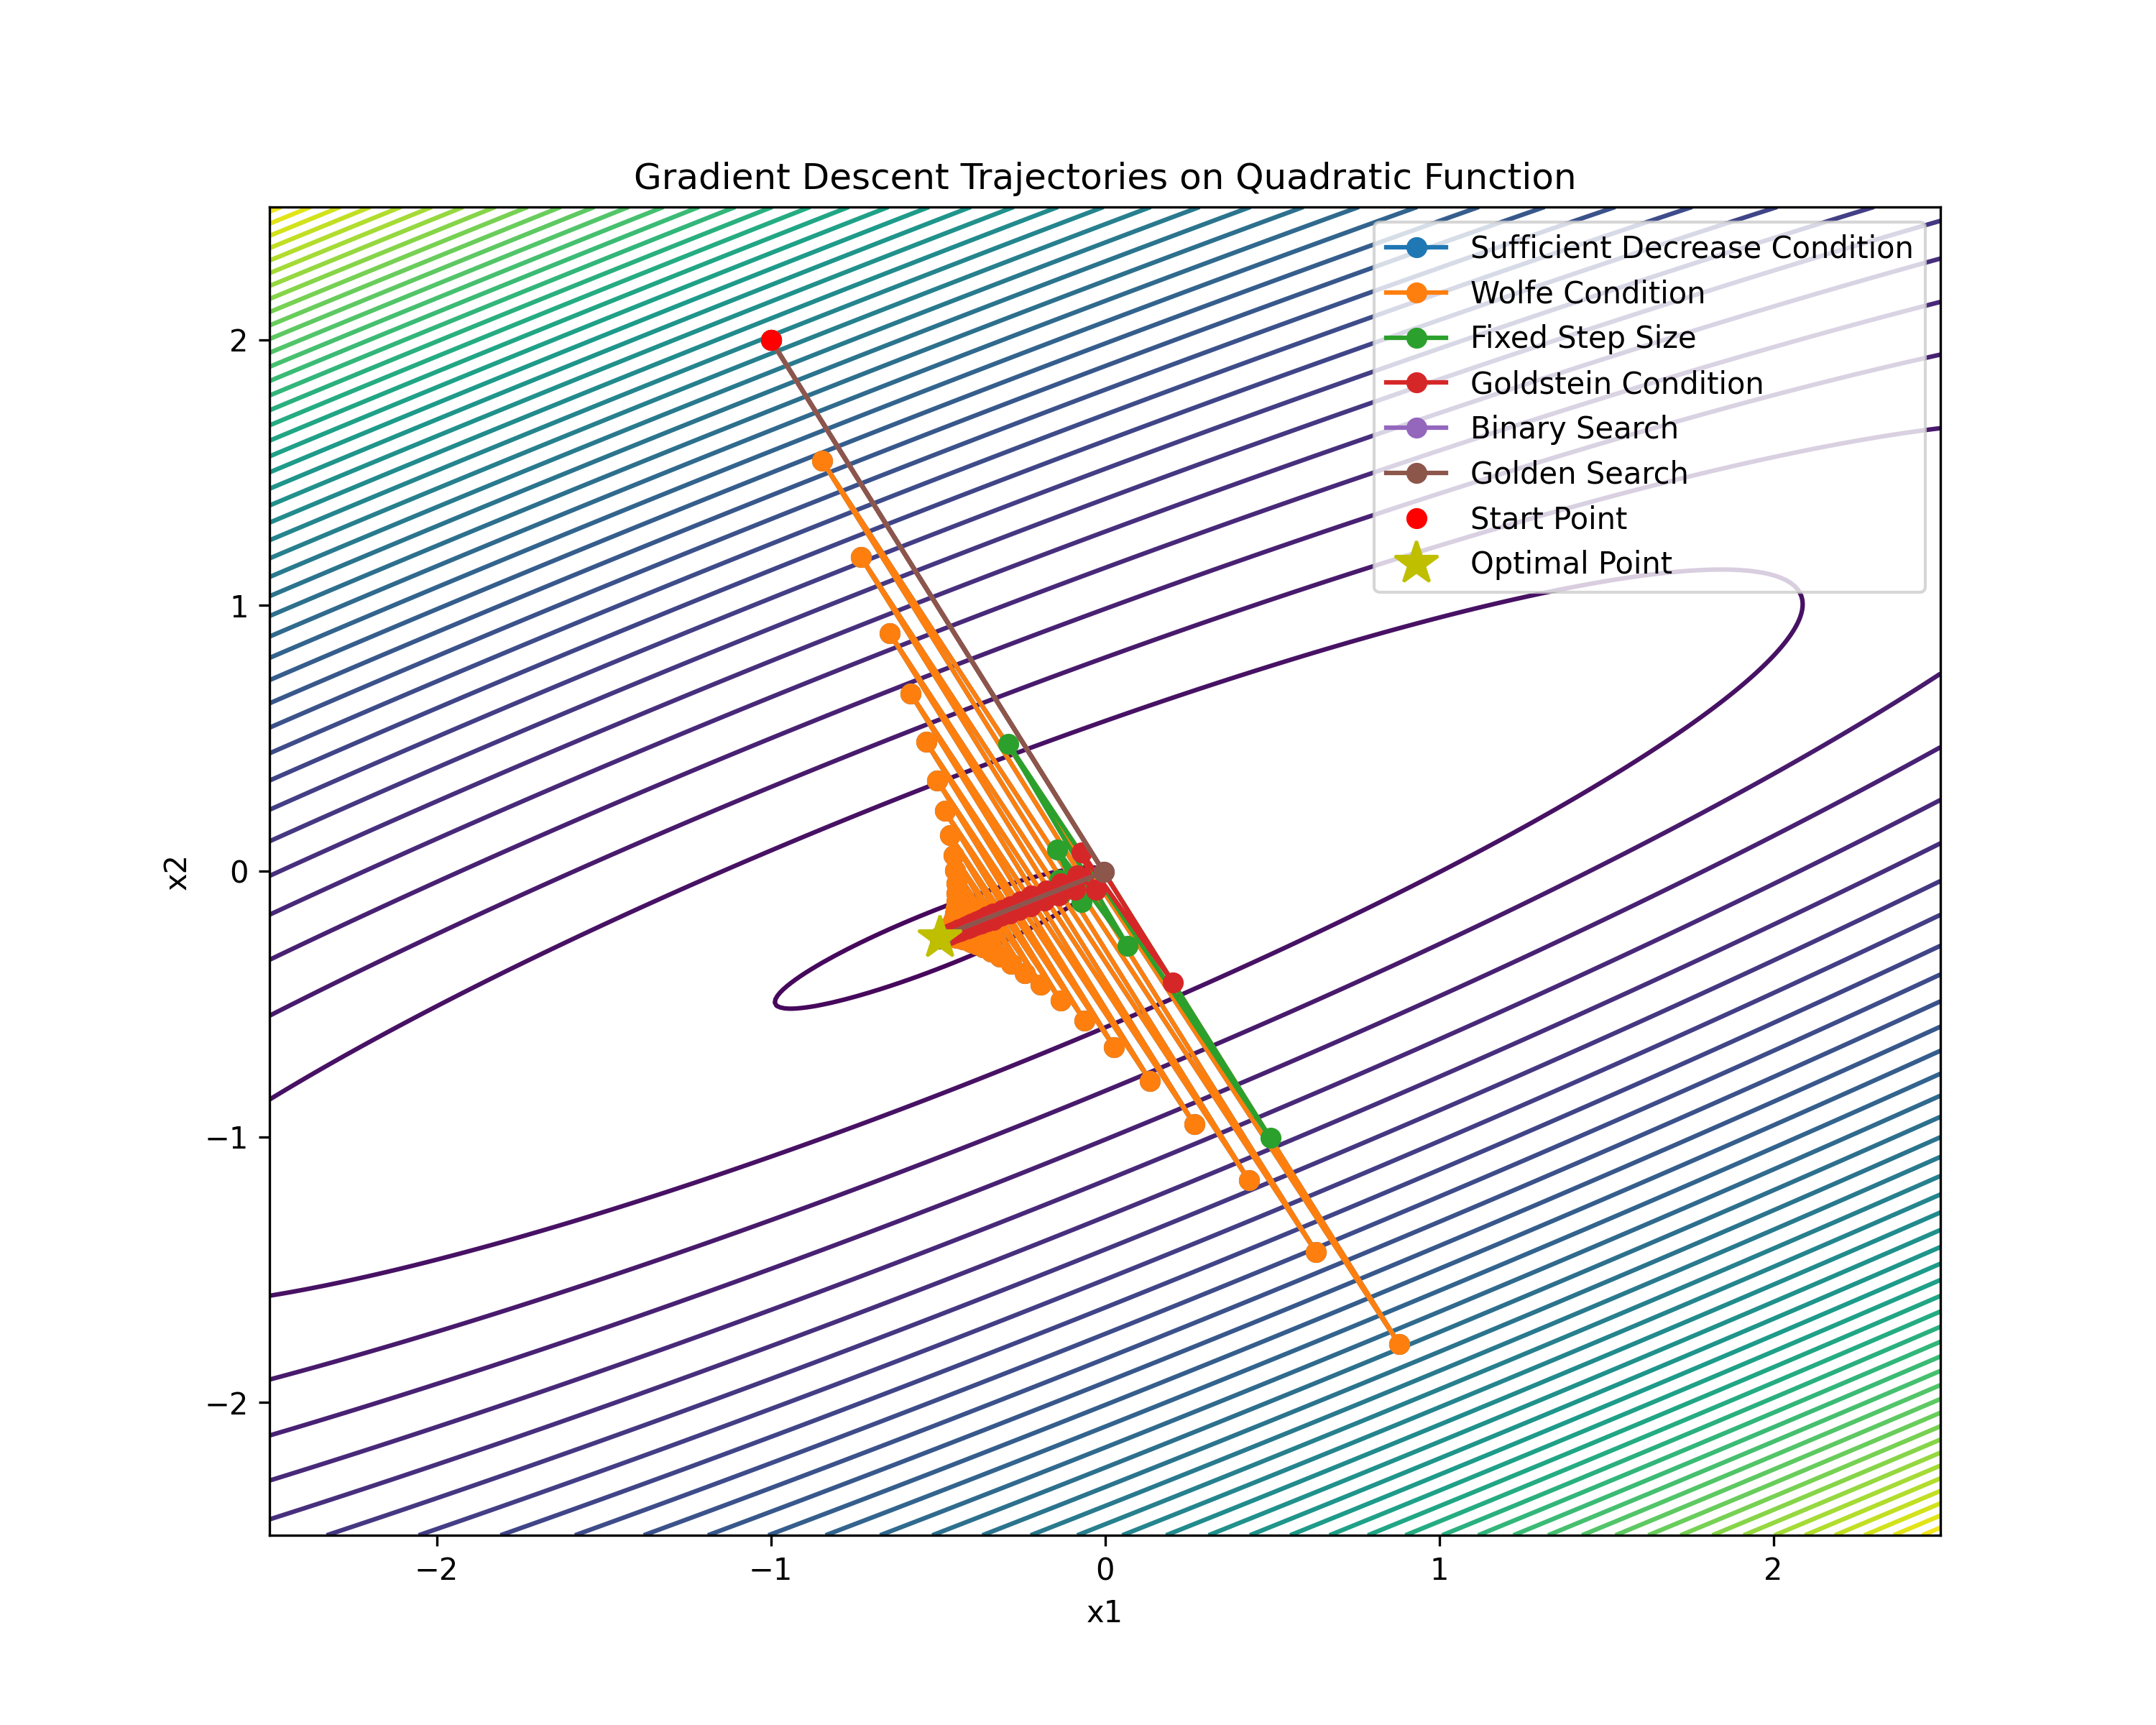
\includegraphics[scale=0.8]{quadratic.png}
\end{figure}

\begin{figure}[H]
    \centering
    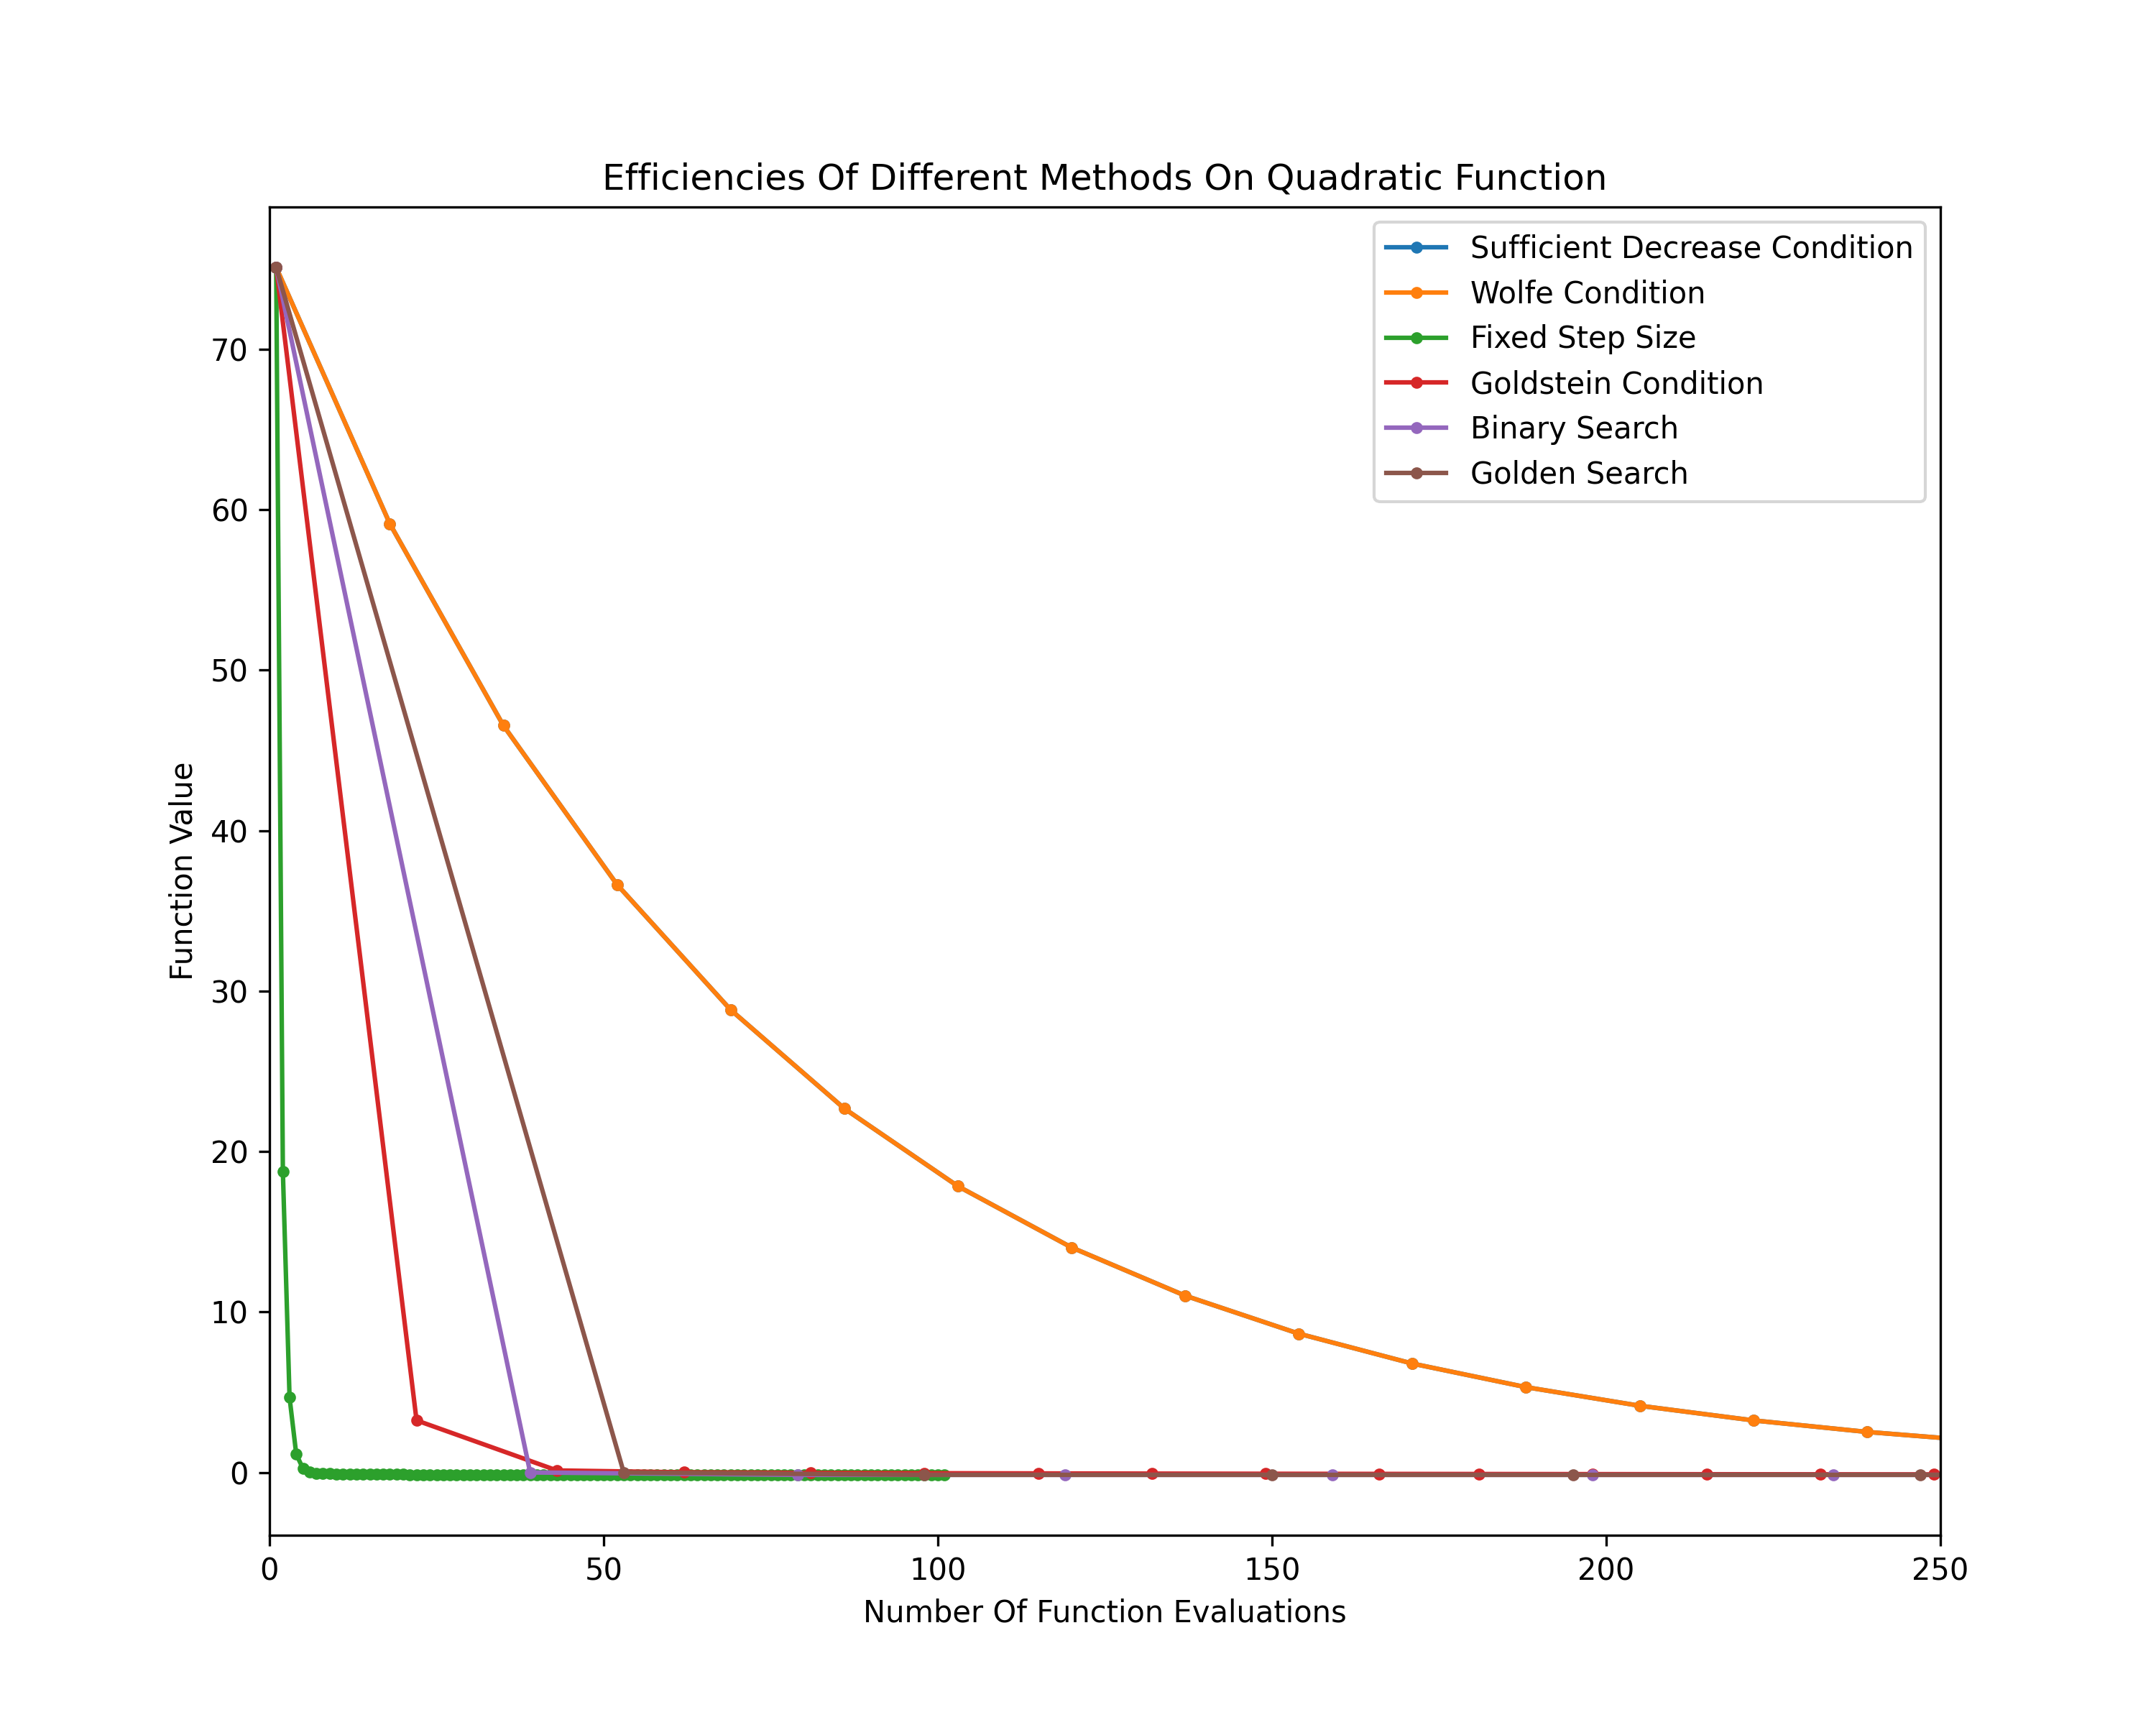
\includegraphics[scale=0.8]{quadratic_efficiencies.png}
\end{figure}

\begin{figure}[H]
    \centering
    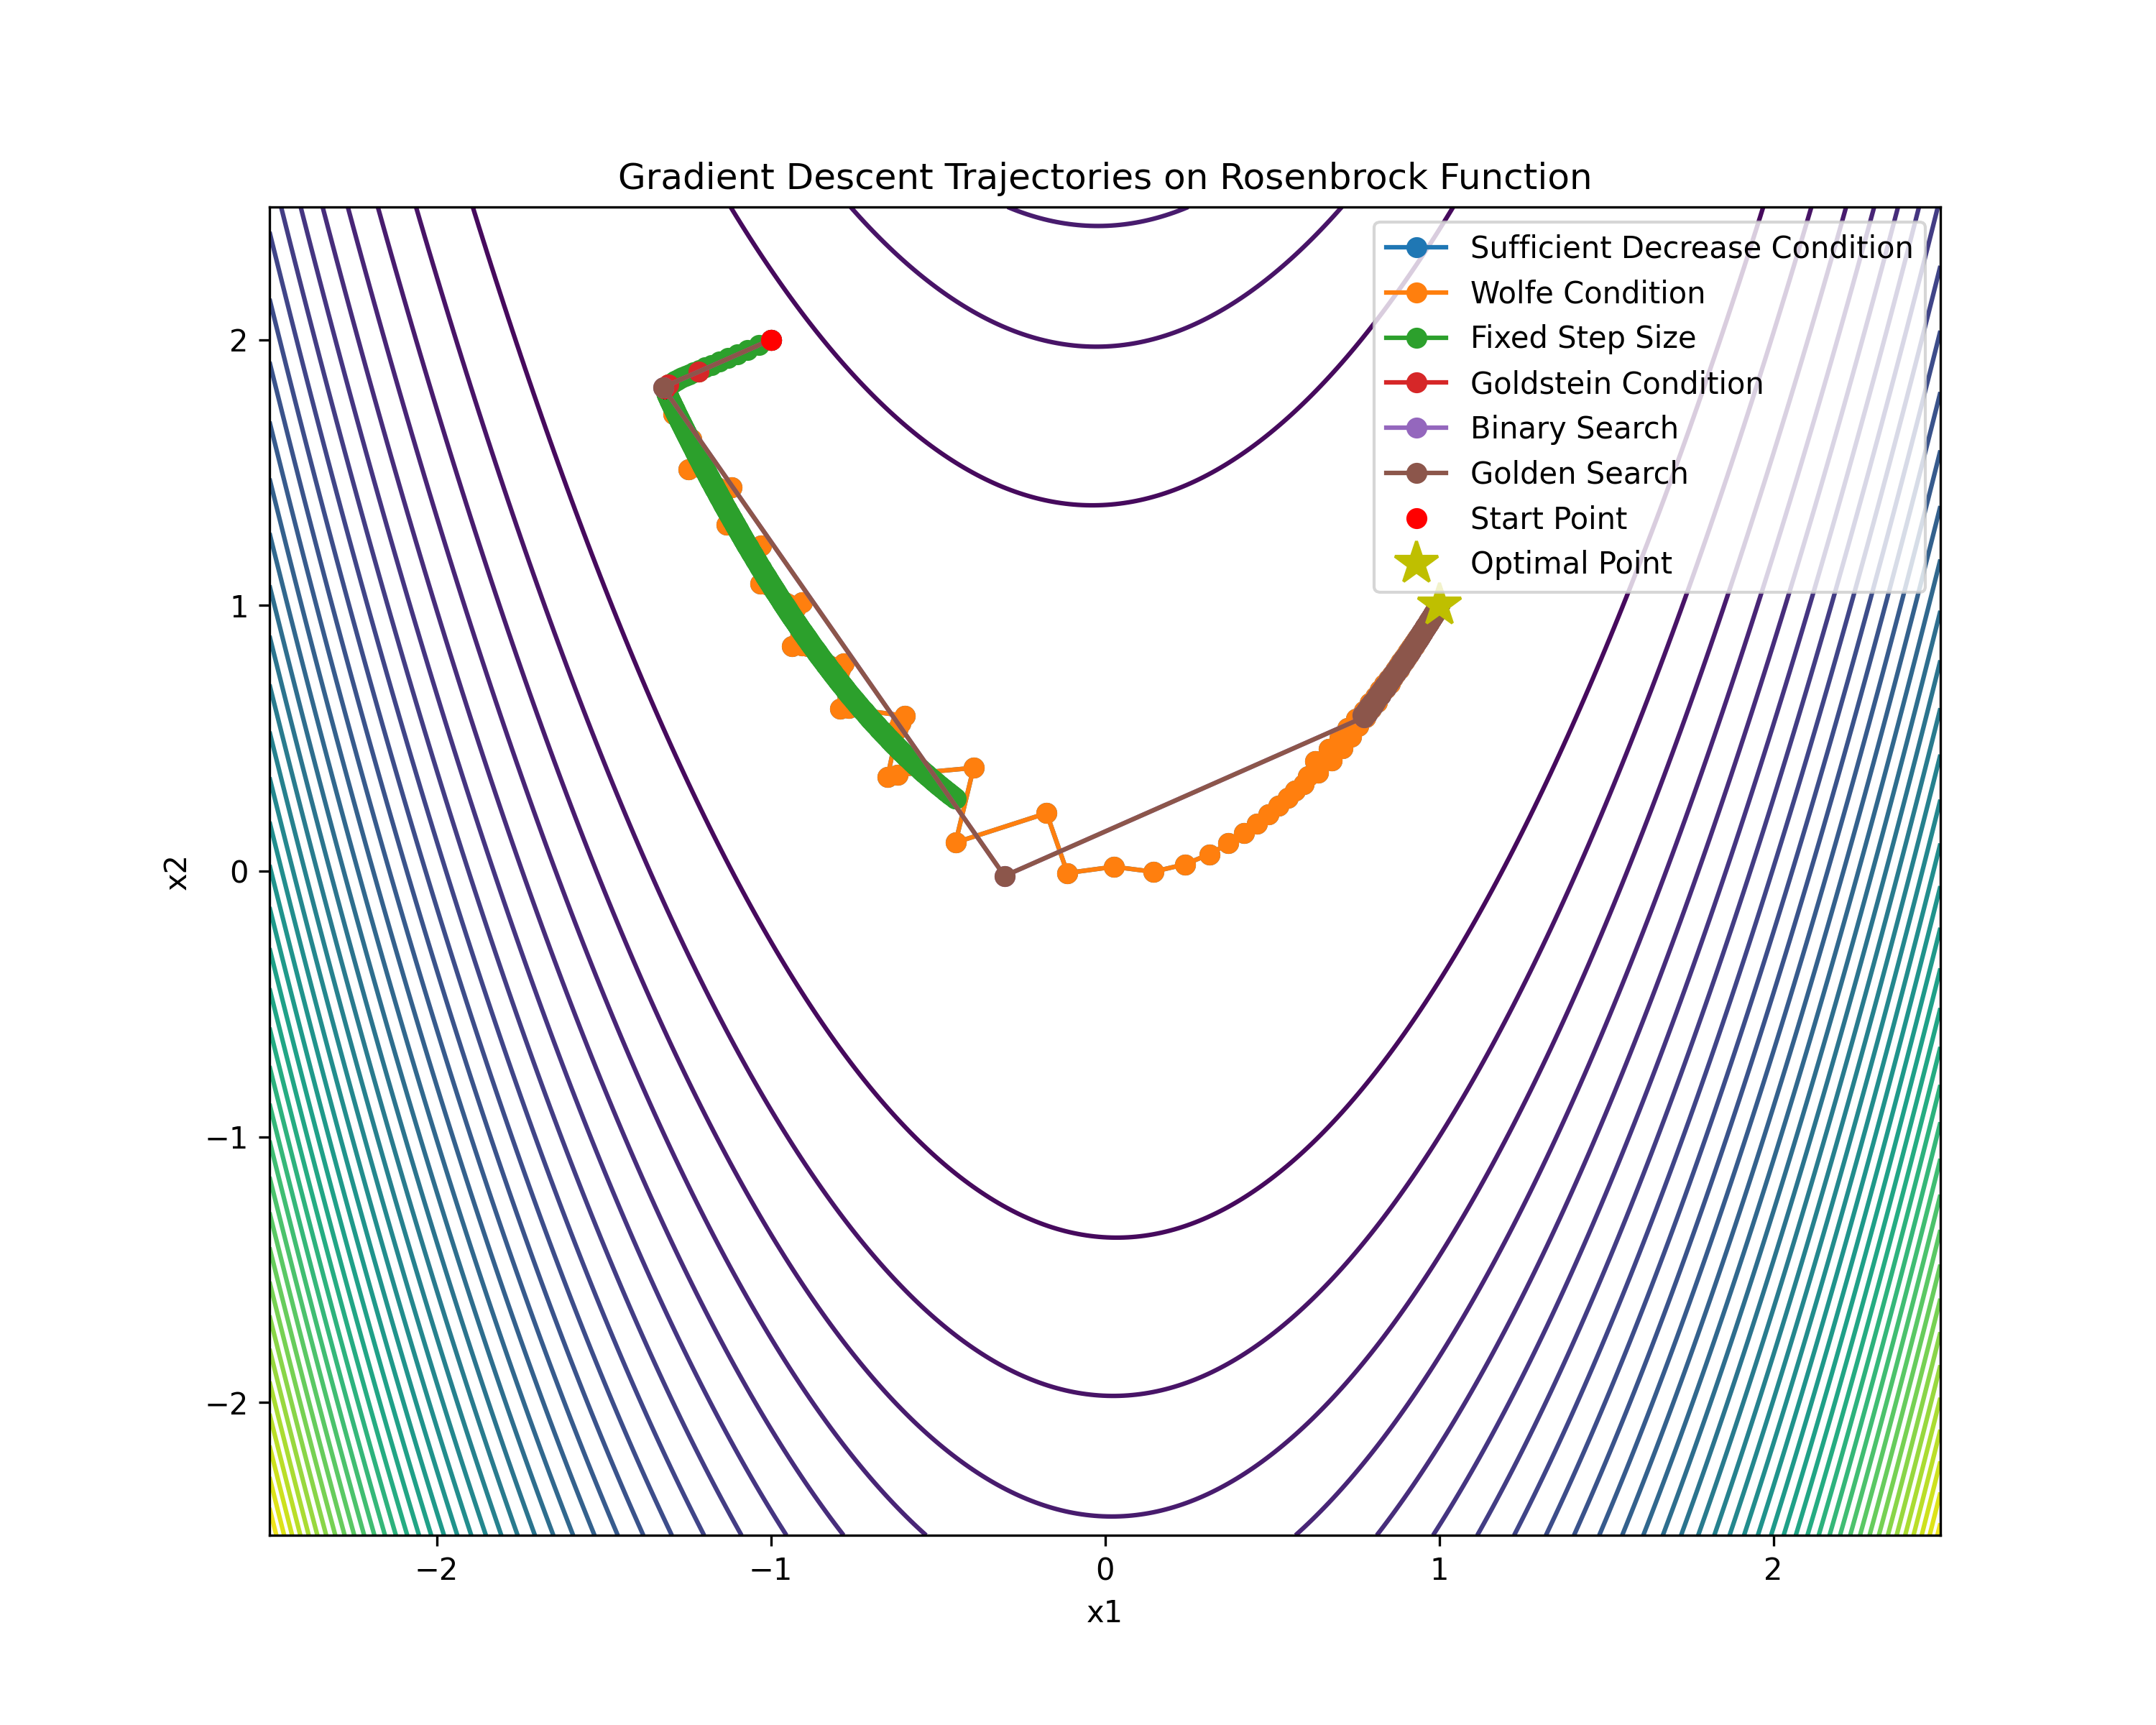
\includegraphics[scale=0.8]{rosenbrock.png}
\end{figure}

\begin{figure}[H]
    \centering
    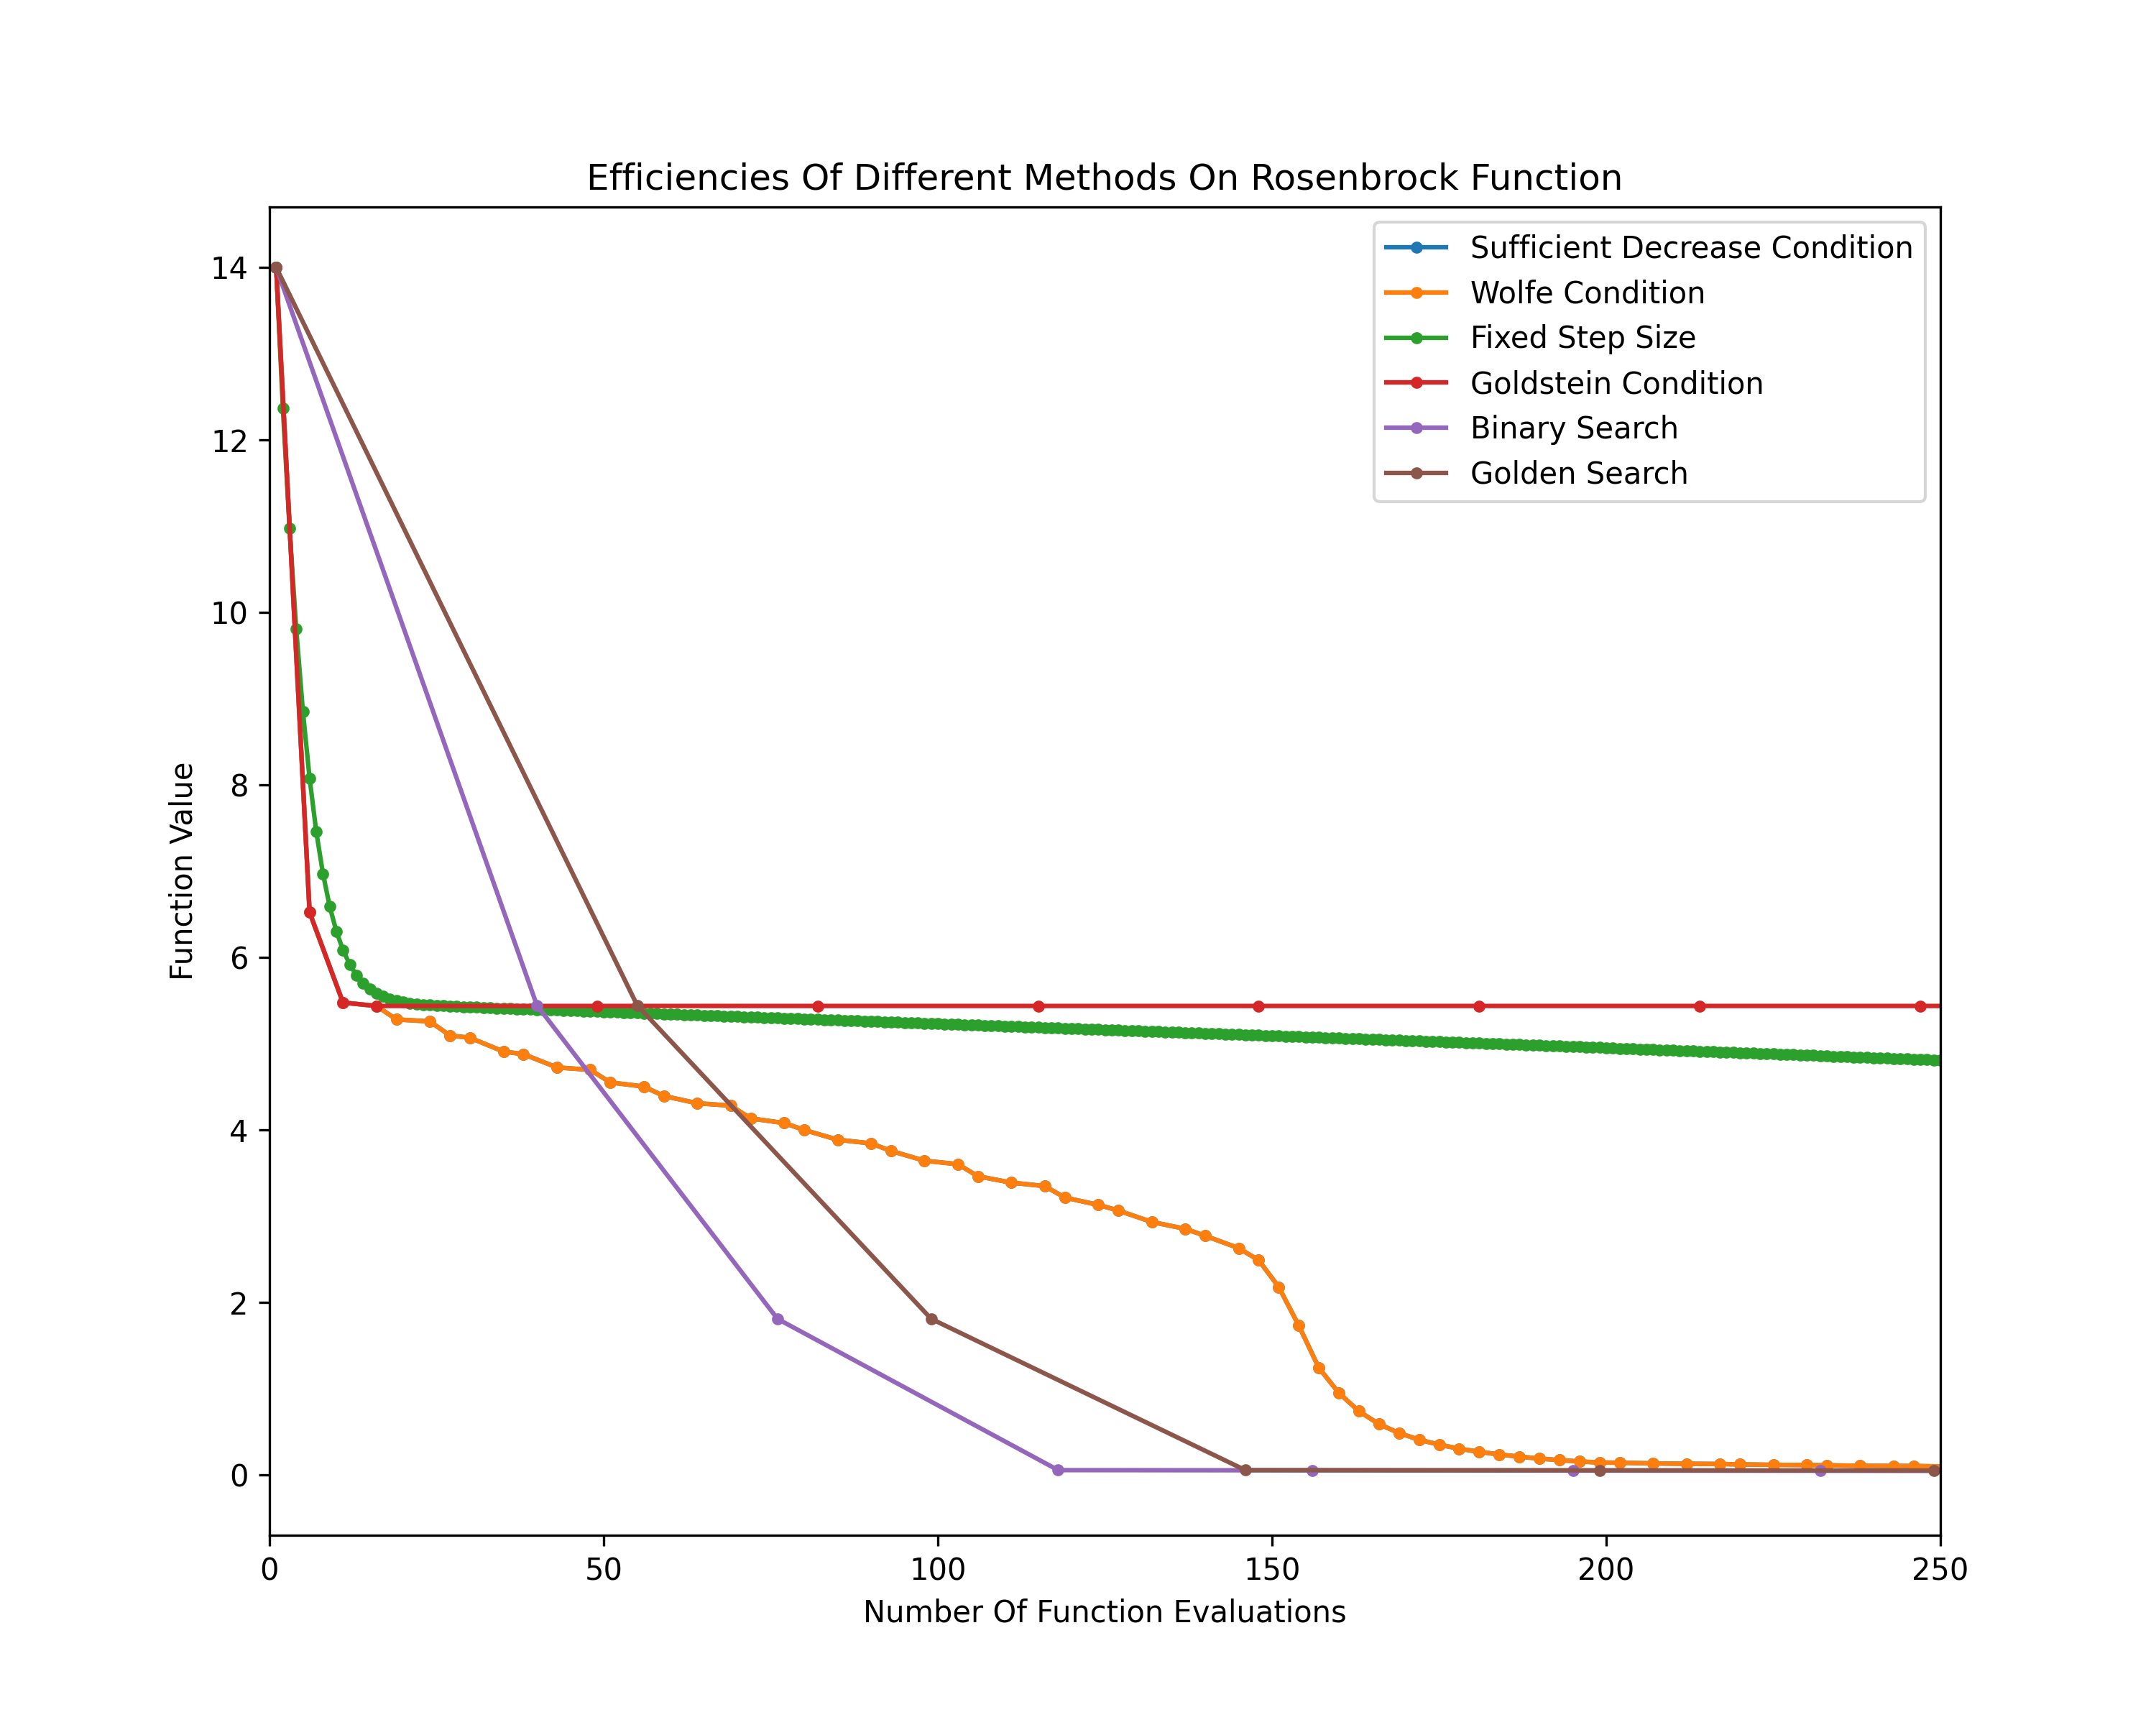
\includegraphics[scale=0.8]{rosenbrock_efficiencies.png}
\end{figure}
%-----------------------------------------------------------------------

\title{Zero order methods}
\maketitle
\paragraph{1.}
\paragraph{2.}

\end{document}

